	\section{Desarrollo de la aplicación móvil}
	Despues de la etapa de construcción, entrenamiento y validación del modelo de reconocimiento de señas, se procedió al desarrollo de la aplicación móvil encargada de integrar el sistema completo dentro de un entorno funcional orientado al usuario final. Esta fase tuvo como objetivo trasladar el pipeline desarrollado en escritorio hacia un dispositivo Android capaz de ejecutar inferencia local de manera continua, utilizando la cámara del dispositivo como fuente de entrada.
	
	A diferencia del entorno experimental, donde las pruebas se realizaron bajo condiciones controladas y utilizando herramientas de análisis y depuración propias del desarrollo en Python, la implementación móvil implicó enfrentar restricciones adicionales relacionadas con rendimiento, consumo de recursos, variabilidad de hardware, orientación del dispositivo y estabilidad del flujo de captura continuo. Por esta razón, la aplicación fue diseñada bajo un enfoque modular, permitiendo separar claramente las responsabilidades asociadas a la captura de imágenes, extracción de landmarks, procesamiento de características, ejecución del modelo e interacción con la interfaz gráfica.
	
	La aplicación fue desarrollada para la plataforma Android utilizando Android Studio como entorno principal de implementación. Ademas se emplearon tecnologías especializadas para cada etapa del pipeline, incluyendo CameraX para la captura continua de imágenes, MediaPipe Hands para la detección y extracción de landmarks de la mano, y TensorFlow Lite para la ejecución del modelo entrenado directamente sobre el dispositivo móvil. Esta integración permitió construir un sistema  funcional capaz de operar sin conexión a internet y con baja latencia de respuesta.
	
	También se realizaron múltiples pruebas orientadas a mejorar la estabilidad del reconocimiento bajo condiciones reales de uso. Entre los principales retos abordados se encontraron las diferencias entre la inferencia realizada en computadora y la inferencia móvil, las variaciones provocadas por cambios de orientación del dispositivo, la necesidad de suavizar predicciones inestables y la optimización del flujo de procesamiento para evitar sobrecarga computacional en dispositivos Android.
	
	Otro aspecto importante fue la implementación de mecanismos de validación temporal y control de estados buscando reducir falsos positivos y mejorar la estabilidad visual del sistema en la interacción continua con el usuario. Estas estrategias permitieron que el reconocimiento no dependiera únicamente de una predicción aislada, sino del análisis consistente de múltiples cuadros consecutivos antes de confirmar una seña detectada.
	
	Las siguientes subsecciones describen la arquitectura general de la aplicación, el flujo de captura y procesamiento de imágenes, la integración del modelo TensorFlow Lite, las estrategias de optimización implementadas y el diseño de la interfaz gráfica utilizada en el prototipo final.
		
	\subsection{Arquitectura general de la aplicación}
	
	Desde el punto de vista de arquitectura de sistema, el prototipo fue desarrollado como una aplicación móvil nativa ejecutada completamente de manera local sobre dispositivos Android. El sistema no depende de servidores externos ni de una arquitectura cliente-servidor, debido a que tanto el procesamiento de visión por computadora como la inferencia del modelo de reconocimiento se realizan directamente en el dispositivo móvil sin necesidad de conexión a internet. Este enfoque permite reducir la latencia del sistema, evitar la dependencia de conectividad y mantener un funcionamiento autónomo del prototipo.
	
	Para la organización interna de la aplicación se adoptó el patrón arquitectónico MVVM (\textit{Model--View--ViewModel}), ampliamente utilizado en aplicaciones Android modernas debido a su capacidad para separar la lógica de presentación, la interfaz gráfica y el manejo de datos. De acuerdo con Microsoft, el patrón MVVM permite desacoplar la lógica de negocio respecto a la interfaz de usuario, facilitando el mantenimiento, reutilización y evolución del software \cite{microsoft_mvvm}. De manera similar, la documentación oficial de Android recomienda arquitecturas desacopladas y organizadas en capas para mejorar la robustez, mantenibilidad y escalabilidad de las aplicaciones móviles \cite{android_architecture}.
	
	Dentro de esta arquitectura, la capa \textit{View} está representada por las pantallas desarrolladas mediante Jetpack Compose, encargadas de mostrar la información al usuario y gestionar la interacción visual. La capa \textit{Model} agrupa los componentes relacionados con la persistencia de datos, el procesamiento de landmarks y la inferencia de modelos de aprendizaje profundo. Finalmente, la capa \textit{ViewModel} administra la lógica de estado, implementa los mecanismos de control temporal y coordina el flujo de reconocimiento, exponiendo los datos de manera asíncrona para actualizar la interfaz gráfica sin comprometer el rendimiento del hilo principal.
	
	Además del patrón MVVM, la aplicación fue organizada bajo una arquitectura modular orientada a separar las distintas responsabilidades asociadas al flujo de captura, procesamiento e inferencia del sistema. Esto permitió mantener una organización clara entre los componentes encargados de la adquisición de imágenes, extracción de características, ejecución del modelo y visualización de resultados, facilitando tanto la depuración como la escalabilidad futura del prototipo.
	
	Debido a que el sistema realiza procesamiento continuo sobre la entrada de la cámara, fue necesario estructurar el flujo interno de manera eficiente para evitar bloqueos en la interfaz gráfica y mantener una experiencia de uso fluida. Por otro lado la separación de componentes permitió desacoplar el procesamiento de visión por computadora respecto a la lógica de interacción con el usuario, reduciendo la complejidad general de la aplicación.
	
	La arquitectura implementada integra tecnologías especializadas para cada etapa del pipeline. CameraX se emplea para la captura continua de imágenes desde la cámara del dispositivo; MediaPipe Hands se encarga de la detección de la mano y extracción de landmarks; TensorFlow Lite realiza la inferencia del modelo de clasificación; y finalmente, la interfaz gráfica muestra el resultado reconocido y administra la interacción visual con el usuario.
	
	La Figura \ref{fig:arquitectura_app} muestra la arquitectura general del prototipo desarrollado. En ella se representa el flujo principal del sistema, comenzando desde la captura de imágenes mediante la cámara del dispositivo hasta la visualización del resultado interpretado por el modelo de reconocimiento.
	
	Primero la imagen capturada es procesada para adecuarla al formato requerido por el modelo de clasificación. Después, el modelo realiza la clasificación correspondiente y el resultado obtenido es mostrado al usuario a través de la interfaz gráfica de la aplicación.
	
	Si bien esta representación resume el funcionamiento general del prototipo, en la implementación móvil fue necesario incorporar componentes adicionales relacionados con la extracción de landmarks, validación temporal, control del flujo continuo de clasificación y estabilización de predicciones, los cuales forman parte de la arquitectura interna final de la aplicación Android.
	
	\begin{figure}[H]
		\centering
		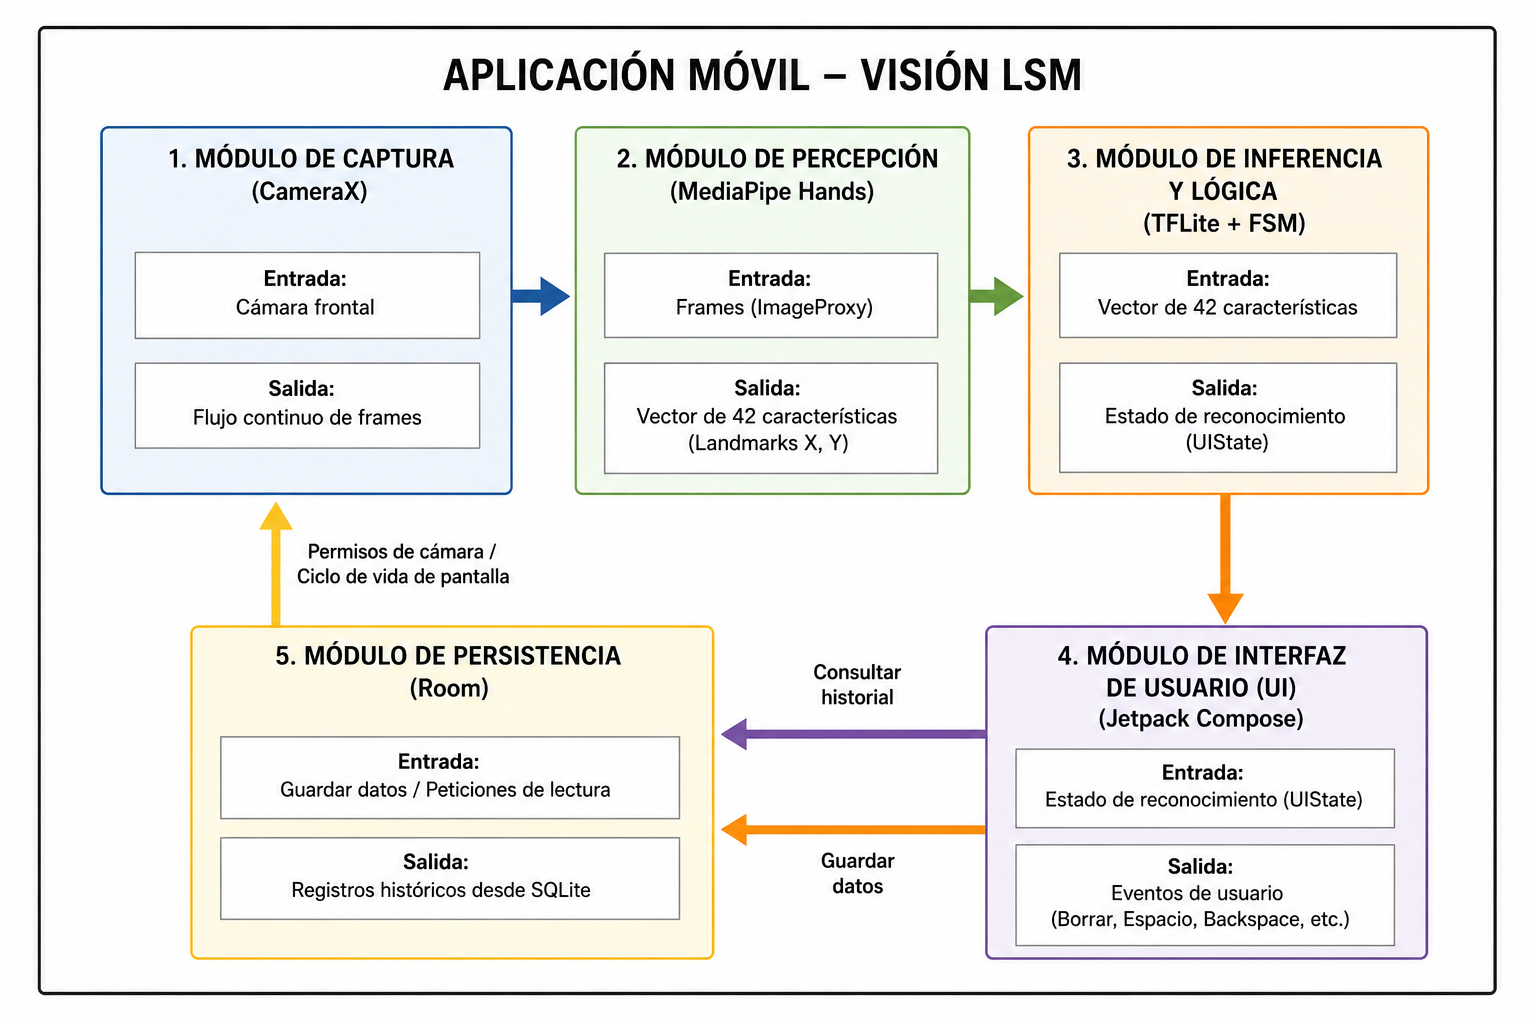
\includegraphics[width=0.8\textwidth]{images/arquitectura_app.png}
		\caption{Arquitectura de la aplicación.}
		\label{fig:arquitectura_app}
	\end{figure}
	
	Como se observa en la Figura \ref{fig:arquitectura_app}, la arquitectura de la aplicación móvil se organizó en cinco módulos principales: captura, percepción, inferencia y lógica, interfaz de usuario y persistencia. Esta división permite separar el funcionamiento interno del sistema de acuerdo con la responsabilidad de cada componente, alineándose de forma directa con los principios del patrón MVVM seleccionado.
	
	El primer componente corresponde al módulo de captura, implementado mediante CameraX. Este módulo recibe como entrada la señal proveniente de la cámara frontal del dispositivo y genera como salida un flujo continuo de frames, representados internamente como objetos \texttt{ImageProxy}. Estos frames son enviados al módulo de percepción para su análisis posterior.
	
	El módulo de percepción utiliza MediaPipe Hands para procesar los frames recibidos, actuando como parte de la capa \textit{Model}. Su función principal es detectar la presencia de la mano dentro de la imagen y obtener los landmarks correspondientes. A partir de estos puntos clave se construye un vector de 42 características, formado por las coordenadas \texttt{x} y \texttt{y} de los 21 landmarks detectados. Este vector representa la configuración geométrica de la mano y   la entrada del modelo de clasificación.
	
	El módulo de inferencia y lógica se comporta como el \textit{ViewModel} central del sistema. Este recibe el vector de características generado por MediaPipe y lo procesa mediante el modelo TensorFlow Lite integrado en la aplicación. Este módulo no solo obtiene la predicción de la seña, sino que también incorpora una máquina de estados encargada de validar la estabilidad temporal del resultado. De esta manera la aplicación evita registrar predicciones aisladas o inestables y únicamente actualiza el estado de reconocimiento expuesto cuando la seña se mantiene durante un periodo suficiente.
	
	El módulo de interfaz de usuario representa la capa \textit{View} y fue desarrollado con Jetpack Compose. Este componente recibe como entrada el estado de reconocimiento expuesto por el \textit{ViewModel}. A partir de este flujo de datos, la pantalla muestra la letra detectada, el texto acumulado, la barra de progreso, los mensajes de estado y los controles de interacción. Además, este módulo permite que el usuario realice acciones como borrar el texto completo, agregar espacios o eliminar la última letra reconocida.
	
	El módulo de persistencia se implementó mediante Room, complementando la capa \textit{Model} para la administración de información local. Este componente recibe solicitudes de guardado o lectura desde la interfaz de usuario y devuelve registros históricos almacenados en SQLite. Su incorporación permite extender el funcionamiento del prototipo hacia funciones como historial de traducciones o almacenamiento de frases reconocidas.
	
	En conjunto esta arquitectura permite que el sistema mantenga un flujo claro entre la captura de imágenes, la extracción de características, la inferencia del modelo y la presentación del resultado final. La separación modular facilita la depuración, el mantenimiento y la posible incorporación de nuevas funcionalidades en versiones futuras del prototipo.
	
	\begin{figure}[H]
		\centering
		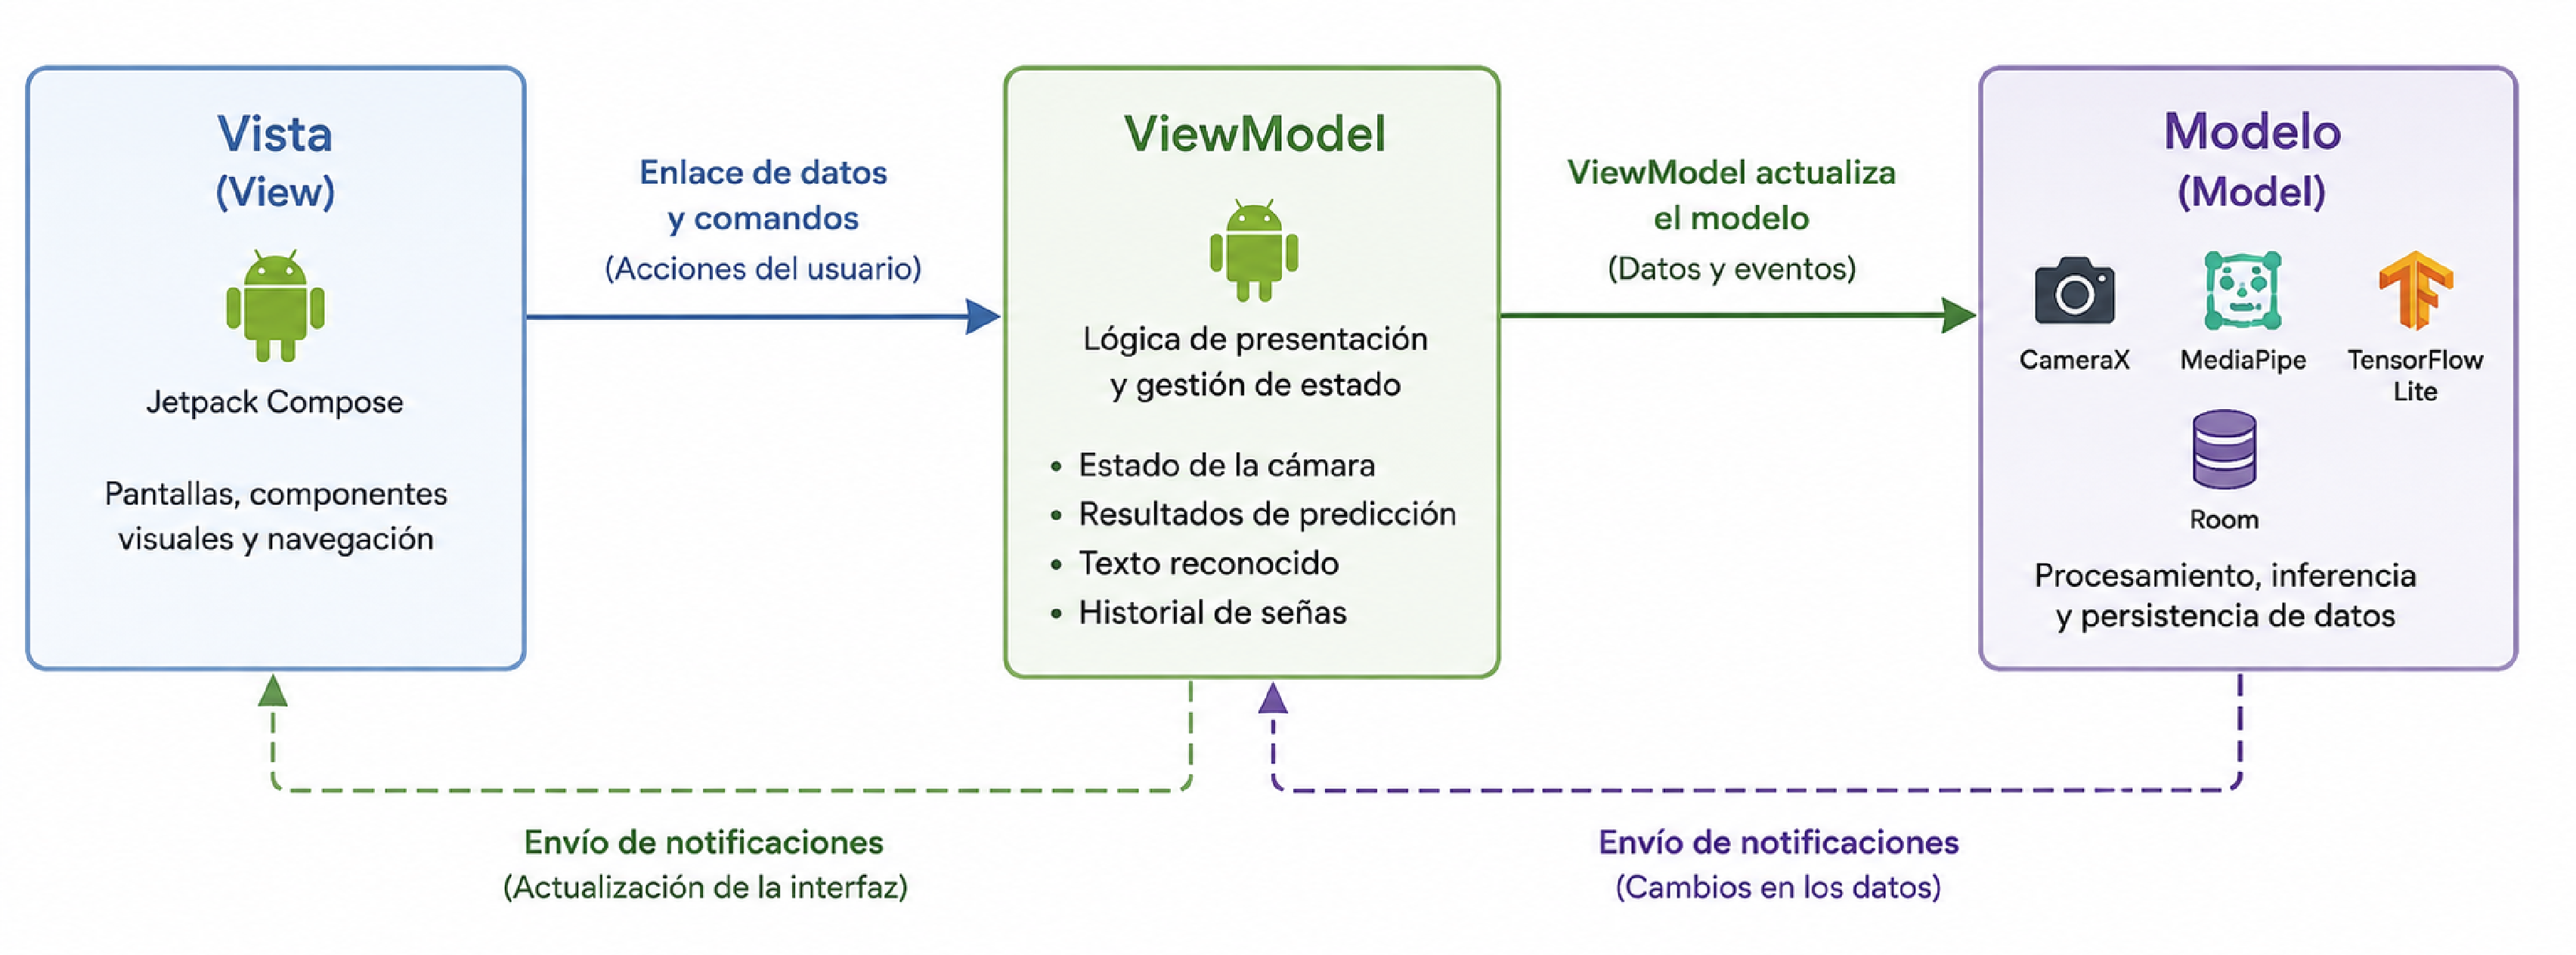
\includegraphics[width=1\textwidth]{images/MVVM.png}
		\caption{MVVM.}
		\label{fig:MVVM}
	\end{figure}

	
	\subsection{Captura de imágenes mediante CameraX}
	
	
	La captura de imágenes dentro de la aplicación móvil se implementó utilizando CameraX, una librería perteneciente a Android Jetpack diseñada para simplificar el acceso y administración de la cámara en dispositivos Android \cite{android_camerax}. CameraX proporciona una capa de abstracción sobre la API Camera2, permitiendo desarrollar aplicaciones con menor complejidad y con mayor compatibilidad entre distintos fabricantes y versiones del sistema operativo Android.
	
	De acuerdo con la documentación oficial de Android Developers, CameraX fue diseñada para resolver problemas comunes asociados al manejo tradicional de cámara, tales como diferencias de hardware, rotación del dispositivo, administración del ciclo de vida y sincronización entre captura y procesamiento de imágenes \cite{android_camerax}. Gracias a esta libreria se pueden construir flujos de captura más estables y adecuados para aplicaciones móviles que requieren procesamiento continuo de imágenes.
	
	En este prototipo desarrollado, CameraX se utilizó para administrar la cámara frontal del dispositivo y proporcionar un flujo continuo de frames hacia el sistema de reconocimiento de señas. La integración se realizó principalmente mediante los componentes \texttt{Preview} e \texttt{ImageAnalysis}. El componente \texttt{Preview} permite mostrar en pantalla la vista previa de la cámara, mientras que \texttt{ImageAnalysis} proporciona acceso continuo a cada frame capturado para su procesamiento posterior mediante MediaPipe y TensorFlow Lite.
	
	CameraX fue importante debido a que el sistema requiere capturar múltiples frames por segundo sin bloquear la interfaz gráfica de la aplicación. Para lograrlo, CameraX administra automáticamente aspectos relacionados con el ciclo de vida de la actividad, la orientación del dispositivo y la liberación de recursos de cámara, permitiendo que el procesamiento de inferencia se ejecute de manera más eficiente sobre dispositivos móviles Android.
	
	La Figura \ref{fig:camerax_flujo} muestra el flujo general implementado para la captura y procesamiento inicial de imágenes dentro de la aplicación móvil.
	
	\begin{figure}[H]
		\centering
		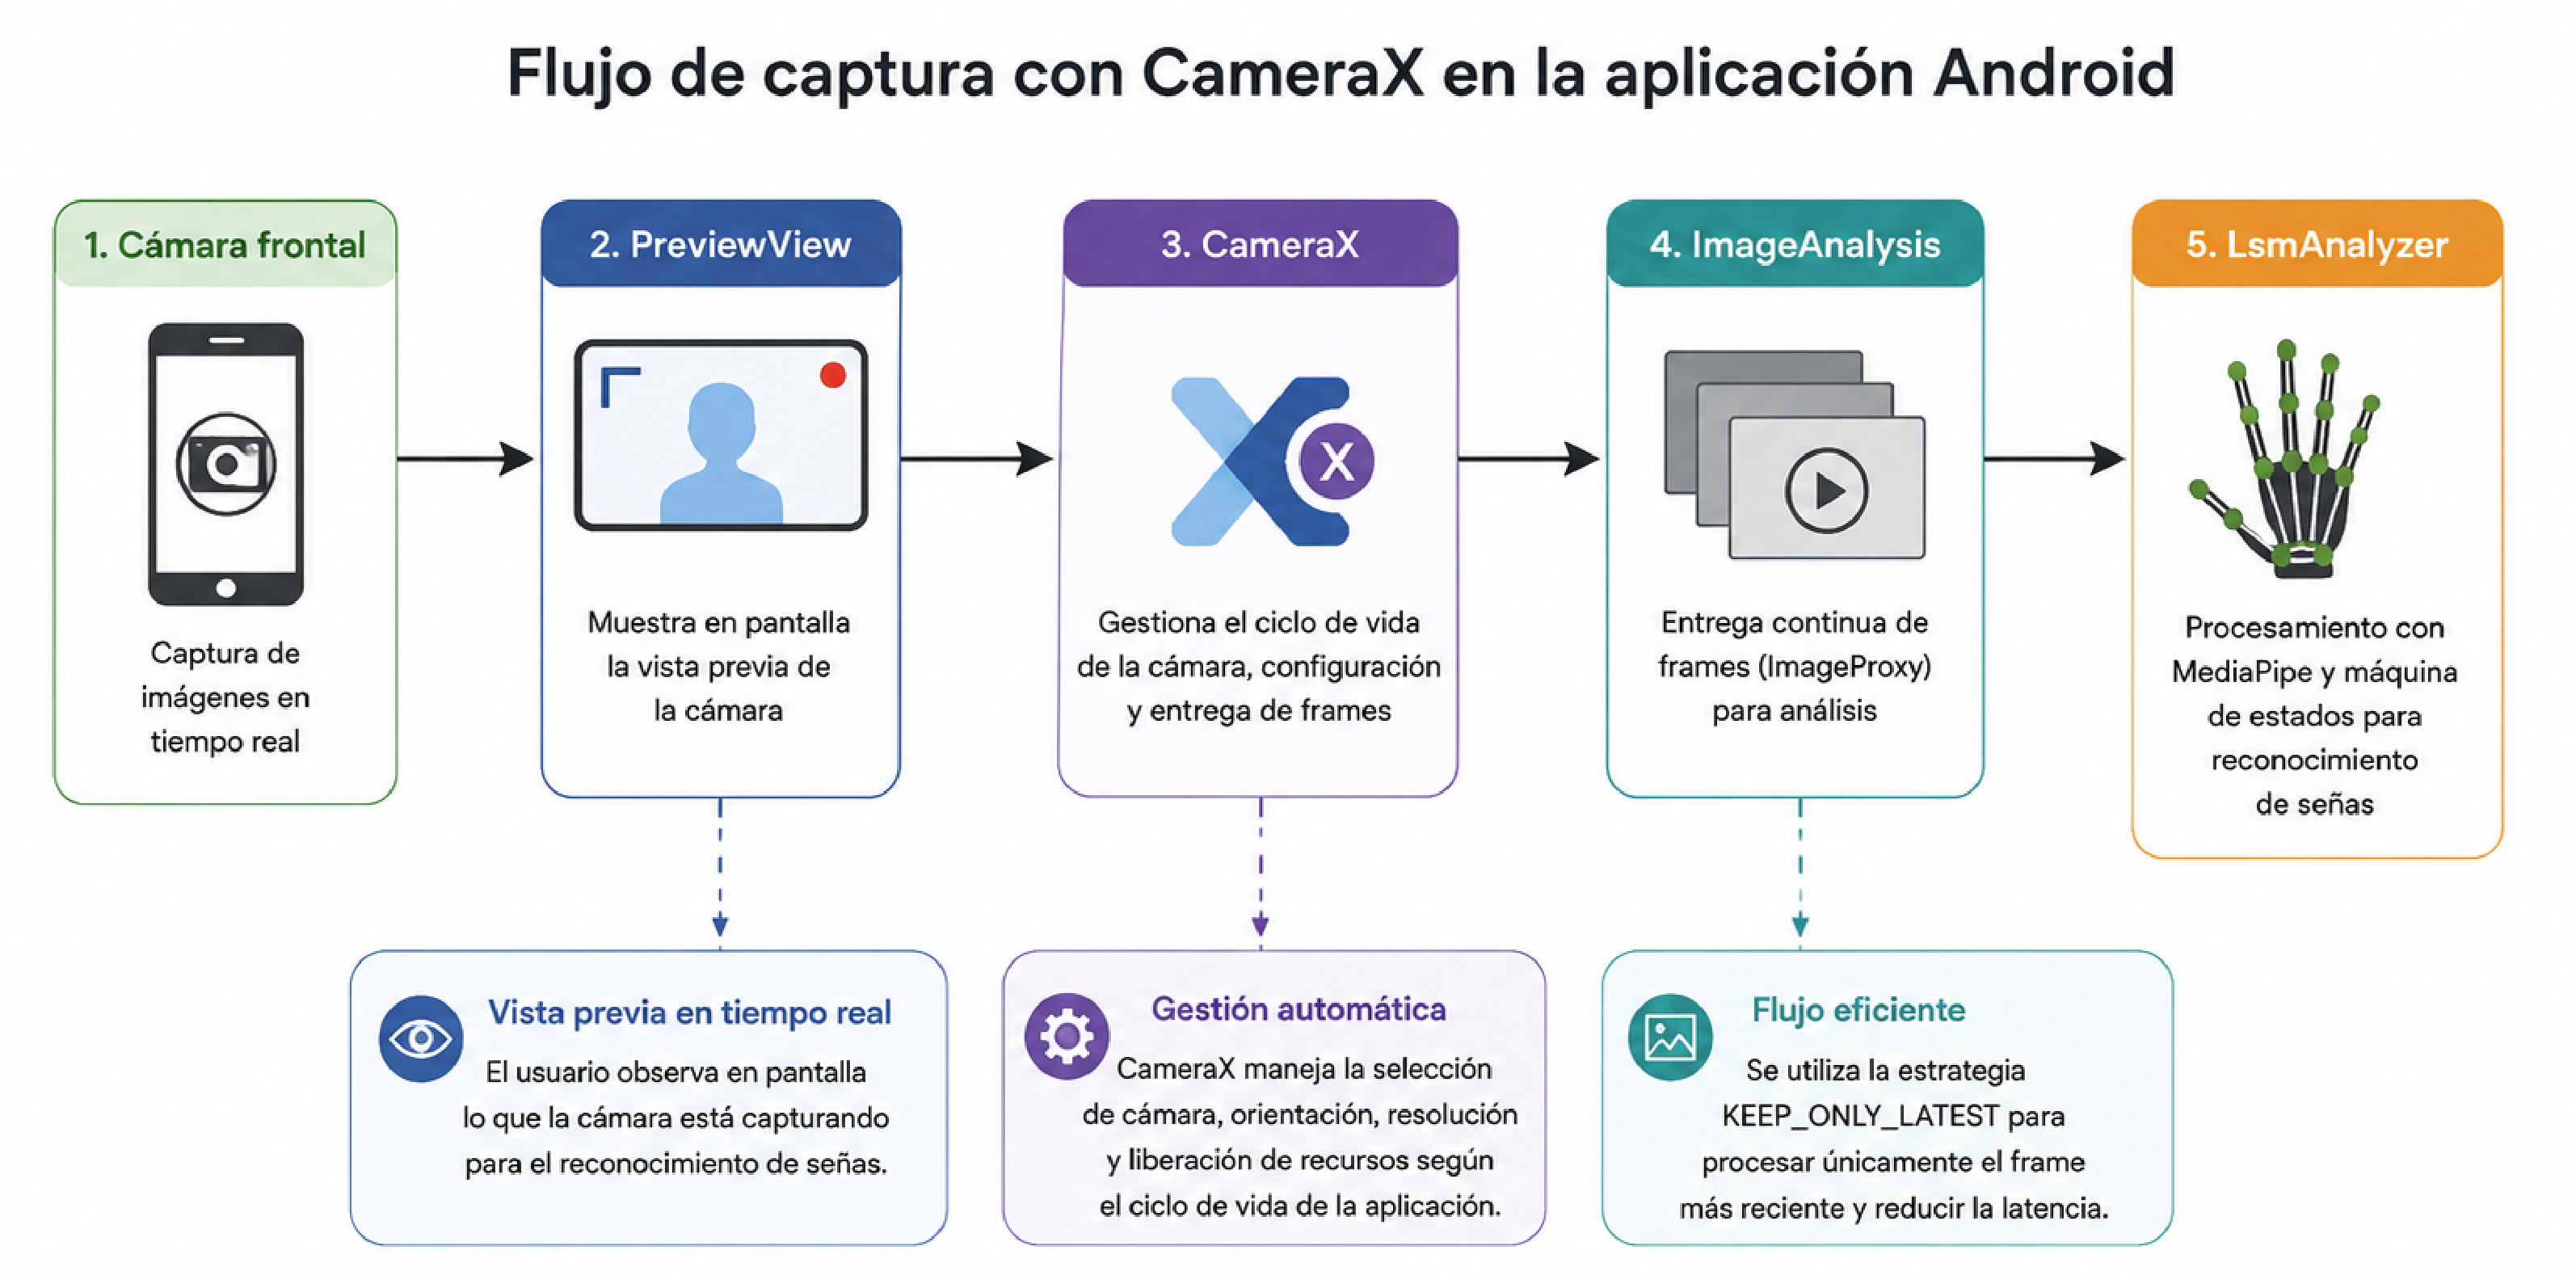
\includegraphics[width=1\textwidth]{images/flujoCamerax.png}
		\caption{Uso de CameraX.}
		\label{fig:camerax_flujo}
	\end{figure}
	
	\begin{algorithm}[H]
		\caption{Inicialización de CameraX y flujo de captura}
		\label{alg:camerax}
		
		Inicializar PreviewView\;
		
		Crear ExecutorService para análisis en segundo plano\;
		
		Obtener instancia de ProcessCameraProvider\;
		
		Configurar Preview con relación de aspecto 16:9\;
		
		Configurar ImageAnalysis con resolución 1280x720\;
		
		Definir estrategia KEEP\_ONLY\_LATEST\;
		
		Asignar LsmAnalyzer como analizador de frames\;
		
		Vincular Preview e ImageAnalysis al ciclo de vida\;
		
		Seleccionar cámara frontal del dispositivo\;
		
		Iniciar flujo continuo de captura\;
		
	\end{algorithm}
	
	
	El Algoritmo \ref{alg:camerax} resume el procedimiento general utilizado para inicializar y administrar la captura de imágenes dentro de la aplicación móvil. Inicialmente se crea un componente \texttt{PreviewView}, encargado de mostrar en pantalla la vista previa proveniente de la cámara frontal del dispositivo. Este componente es integrado dentro de la interfaz desarrollada con Jetpack Compose mediante \texttt{AndroidView}, permitiendo combinar componentes nativos de Android con la interfaz declarativa de Compose.
	
	Luego, se crea un \texttt{ExecutorService} que se encarga del procesamiento de imágenes en segundo plano. Esto es importante dado que el reconocimiento de señas requiere analizar múltiples frames de manera continua. Si el análisis se ejecutara directamente sobre el hilo principal de la aplicación, la interfaz gráfica podría bloquearse o presentar retrasos perceptibles para el usuario. Al utilizar un hilo independiente la captura y el procesamiento pueden ejecutarse simultáneamente manteniendo una experiencia de uso fluida.
	
	La inicialización de CameraX se realiza mediante \texttt{ProcessCameraProvider}, componente encargado de administrar los recursos de cámara y vincularlos al ciclo de vida de la pantalla. Esto ayuda a que la cámara se active únicamente cuando la pantalla de reconocimiento se encuentra disponible y libera automáticamente sus recursos cuando el usuario abandona dicha pantalla, evitando conflictos internos y consumo innecesario de memoria o batería.
	
	Dentro de la configuración se definieron dos casos de uso principales: \texttt{Preview} e \texttt{ImageAnalysis}. El primero se encarga de enviar la señal visual hacia el \texttt{PreviewView}, permitiendo que el usuario observe la imagen capturada por la cámara. El segundo proporciona acceso continuo a los frames capturados para que puedan ser enviados posteriormente al módulo de análisis de señas.
	
	El componente \texttt{ImageAnalysis} fue configurado con una resolución de \texttt{1280x720} píxeles y una relación de aspecto de \texttt{16:9}. Esta configuración permite mantener un equilibrio entre calidad visual y rendimiento computacional, proporcionando imágenes suficientemente detalladas para la detección de la mano sin incrementar excesivamente el costo de procesamiento sobre el dispositivo móvil.
	
	Se configuró la estrategia \texttt{ImageAnalysis.STRATEGY\_KEEP\_ONLY\_LATEST}, la cual indica a CameraX que si el analizador no puede procesar todos los frames al mismo ritmo en que son capturados, únicamente se conserve el frame más reciente y se descarten los pendientes en la cola de procesamiento, ya que es preferible analizar información actualizada del usuario en lugar de acumular imágenes atrasadas que incrementarían la latencia de la aplicación.
	
	Los componentes \texttt{Preview} e \texttt{ImageAnalysis} son vinculados al ciclo de vida de la pantalla mediante \texttt{bindToLifecycle()}, seleccionando la cámara frontal del dispositivo. La cámara frontal fue elegida debido a que proporciona una interacción más natural para el usuario, permitiéndole observar su posición en pantalla mientras realiza las señas y recibir retroalimentación visual inmediata del sistema.
	
	El módulo de captura cumple dos funciones simultáneas. Por un lado, proporciona una vista previa continua para guiar visualmente al usuario en la interacción. Por otro lado, entrega continuamente los frames capturados al componente \texttt{LsmAnalyzer}, encargado de iniciar el procesamiento de reconocimiento de señas.
	
	En la implementación de este módulo se identificaron múltiples dificultades relacionadas con la orientación del dispositivo móvil y la forma en que android entrega los frames provenientes de la cámara frontal. Inicialmente se asumió que la orientación horizontal habitual del teléfono correspondía a una rotación de \(0^\circ\); sin embargo, en las pruebas experimentales se observó que android maneja internamente distintas referencias de orientación dependiendo del fabricante, la posición física del dispositivo y la cámara utilizada.
	
	Se detectó que al utilizar la cámara frontal en orientación horizontal convencional, el sistema reportaba una rotación de \(270^\circ\), mientras que la orientación \(0^\circ\) aparecía cuando el dispositivo se encontraba físicamente invertido. Esta situación provocaba inconsistencias importantes entre la imagen mostrada al usuario y la orientación real utilizada en el procesamiento de visión por computadora.
	
	En un inicio los frames capturados eran enviados directamente hacia MediaPipe sin aplicar correcciones geométricas adicionales. Como consecuencia, el detector de manos presentaba múltiples fallos: en algunos casos no detectaba ninguna mano dentro de la imagen y, en otros, los landmarks aparecían invertidos o desplazados respecto a la posición observada visualmente en pantalla.
	
	Para resolver este problema fue necesario incorporar una etapa de transformación antes de construir la imagen utilizada por MediaPipe. Cada frame recibido desde CameraX fue convertido inicialmente a un objeto \texttt{Bitmap}, sobre el cual posteriormente se aplicaron transformaciones de rotación y espejo mediante una matriz de transformación. Estas operaciones permitieron corregir tanto la orientación física del dispositivo como el efecto espejo característico de la cámara frontal.
	
	\begin{lstlisting}[language=Java, caption={Corrección de orientación y efecto espejo antes de MediaPipe.}, label={lst:rotation_fix}]
		val matrix = Matrix().apply {
			postRotate(image.imageInfo.rotationDegrees.toFloat())
			postScale(-1f, 1f)
		}
		
		processedBitmap = Bitmap.createBitmap(
		bitmap,
		0,
		0,
		bitmap.width,
		bitmap.height,
		matrix,
		true
		)
	\end{lstlisting}
	
	La instrucción \texttt{postRotate()} permite compensar la orientación reportada por Android, garantizando que la imagen llegue correctamente alineada al detector de MediaPipe. Por otro lado, \texttt{postScale(-1f, 1f)} aplica una inversión horizontal necesaria debido a que la cámara frontal genera una vista espejada para el usuario. Sin esta corrección, las configuraciones geométricas de la mano podían invertirse respecto a las utilizadas en el entrenamiento del modelo.
	
	Después de incorporar estas transformaciones, la detección de landmarks se volvió considerablemente más estable y consistente entre diferentes orientaciones del dispositivo. En las pruebas se observó que la orientación horizontal seguía ofreciendo mejores resultados de reconocimiento en comparación con la orientación vertical. Esto se debía principalmente a diferencias en la distribución espacial de los landmarks y en la forma en que la cámara frontal recortaba el área visible de captura.
	
	Aparte de la orientación, también se presentaron dificultades relacionadas con la relación de aspecto y el escalado de la imagen mostrada en pantalla. Debido a que \texttt{PreviewView} utiliza internamente estrategias de escalado para ajustar la vista previa al tamaño de la interfaz, las coordenadas normalizadas obtenidas por MediaPipe no coincidían directamente con la posición visual mostrada al usuario. Dada esta situación, fue necesario implementar funciones adicionales de mapeo geométrico para ajustar correctamente las cajas delimitadoras dibujadas sobre la interfaz.
	
	Todas las variantes y pruebas realizadas demostraron que factores como rotación, orientación, escalado, relación de aspecto y comportamiento de la cámara frontal influyen directamente en la estabilidad del reconocimiento y en la calidad de los landmarks generados posteriormente por MediaPipe.

	
	\subsection{Implementación del analizador de señas}
	
	El analizador de señas es el componente encargado de conectar el flujo de imágenes entregado por CameraX con el proceso de reconocimiento basado en landmarks y clasificación mediante el modelo entrenado. En la aplicación este componente fue implementado mediante la clase \texttt{LsmAnalyzer}, la cual extiende la interfaz \texttt{ImageAnalysis.Analyzer}. Esto hace que cada frame capturado por la cámara pueda ser procesado de manera continua dentro del flujo de análisis de CameraX.
	
	La función principal del analizador consiste en recibir cada imagen en formato \texttt{ImageProxy}, prepararla para ser procesada por MediaPipe Hands, extraer los puntos clave de la mano detectada y transformar dicha información en un vector numérico compatible con el modelo de clasificación. Es por eso que el analizador actúa como un puente entre la captura visual y la etapa de inferencia, ya que convierte información visual cruda en una representación estructurada de la mano.
	
	Para la detección de la mano se utilizó el modelo \texttt{hand\_landmarker.task} de MediaPipe. Este modelo fue configurado en modo \texttt{VIDEO}, debido a que la entrada del sistema no corresponde a una imagen aislada, sino a una secuencia continua de frames provenientes de la cámara. Se configuró la detección para una sola mano, considerando que el prototipo se orientó al reconocimiento de señas estáticas realizadas con una mano. También se establecieron umbrales mínimos de detección, presencia y seguimiento para evitar que el sistema procesara resultados demasiado inestables o detecciones incompletas.
	
	El proceso de análisis inicia validando que el analizador se encuentre activo y que el detector de MediaPipe haya sido inicializado correctamente. Esta verificación evita que el sistema intente procesar frames cuando el recurso ya fue cerrado o cuando ocurrió algún error en la carga del modelo de detección de manos. En cualquiera de estos casos, el frame se descarta y se libera inmediatamente para no bloquear el flujo de CameraX.
	
	Despues del proceso anterior cada frame recibido se convierte a un objeto \texttt{Bitmap}. Esta conversión es necesaria porque MediaPipe requiere una imagen compatible con su formato de entrada, representado mediante \texttt{MPImage}. Antes de construir dicha imagen, se aplica una transformación geométrica al frame para corregir la orientación reportada por Android y el efecto espejo generado por la cámara frontal. Este proceso fue importante para asegurar que MediaPipe recibiera la imagen con una orientación coherente y pudiera detectar correctamente la mano.
	
	Una vez que se corrige la imagen se construye el objeto \texttt{MPImage} y se envía al detector mediante el método \texttt{detectForVideo}. El uso de este método requiere proporcionar una marca de tiempo en milisegundos, por lo que se utiliza el \textit{timestamp} del frame entregado por CameraX. Esta marca temporal permite a MediaPipe mantener coherencia en el procesamiento de una secuencia de video, especialmente cuando se trabaja con mecanismos de seguimiento entre frames.
	
	Si MediaPipe no detecta landmarks en el frame analizado, el sistema devuelve un resultado vacío representado por la etiqueta \texttt{"..."} y una confianza igual a cero. Esta salida permite indicar que no existe una seña válida en ese instante, sin interrumpir el flujo continuo de captura. En cambio, cuando se detecta una mano válida, el analizador toma el primer conjunto de landmarks y verifica que contenga al menos 21 puntos clave, correspondientes al modelo estándar de MediaPipe Hands.
	
	A partir de estos landmarks se construye el vector de características utilizado por el clasificador. Para ello, se extraen únicamente las coordenadas \texttt{x} y \texttt{y} de cada punto, generando un total de 42 valores numéricos. Esta decisión se mantiene consistente con el enfoque utilizado en el entrenamiento, donde la representación de la seña se basó en la geometría bidimensional de la mano. Las coordenadas obtenidas son posteriormente normalizadas para reducir la dependencia respecto a la posición y tamaño de la mano dentro del encuadre. El impacto de estas variantes de normalización y su relación con las diferencias entre pruebas en computadora y dispositivo móvil se analiza en la subsección siguiente.
	
	Ya construido el vector de 42 características, este se envía al componente \texttt{LsmClassifier}, encargado de ejecutar el modelo de clasificación. El analizador no interpreta directamente la salida del modelo, sino que delega dicha tarea al clasificador y recibe como resultado una etiqueta y un valor de confianza. Esta separación permite mantener desacopladas las responsabilidades del sistema: el analizador se encarga de preparar la información proveniente de la cámara y el clasificador se encarga de ejecutar la inferencia sobre el modelo entrenado.
	
	El resultado obtenido se envía hacia la interfaz mediante una función de retorno \texttt{onResult}. Esta función permite comunicar la letra detectada y su confianza sin acoplar el analizador directamente a los componentes visuales de la aplicación. Esto permite que el analizador puede operar como un módulo independiente dentro del flujo de reconocimiento, facilitando su depuración, mantenimiento y posible sustitución en versiones futuras.
	
	Es importante señalar que, aunque el analizador entrega una predicción por cada frame procesado, dicha predicción no necesariamente se considera como una letra confirmada por el sistema. La estabilización temporal, el control de falsos positivos y la confirmación final de las señas se abordan posteriormente dentro del flujo general de operación y la lógica de validación del prototipo. 
	
	La Figura~\ref{fig:deteccion-mano-video} resume el flujo seguido por el analizador para procesar cada frame capturado por la cámara. Primero, la imagen es recibida desde CameraX; posteriormente, se corrige su orientación y formato para construir un objeto compatible con MediaPipe. Después, el frame se analiza mediante el método \texttt{detectForVideo}, utilizando una marca temporal que permite mantener la coherencia entre frames y mejorar el seguimiento de la mano en la secuencia de video.
	
	\begin{figure}[H]
		\centering
		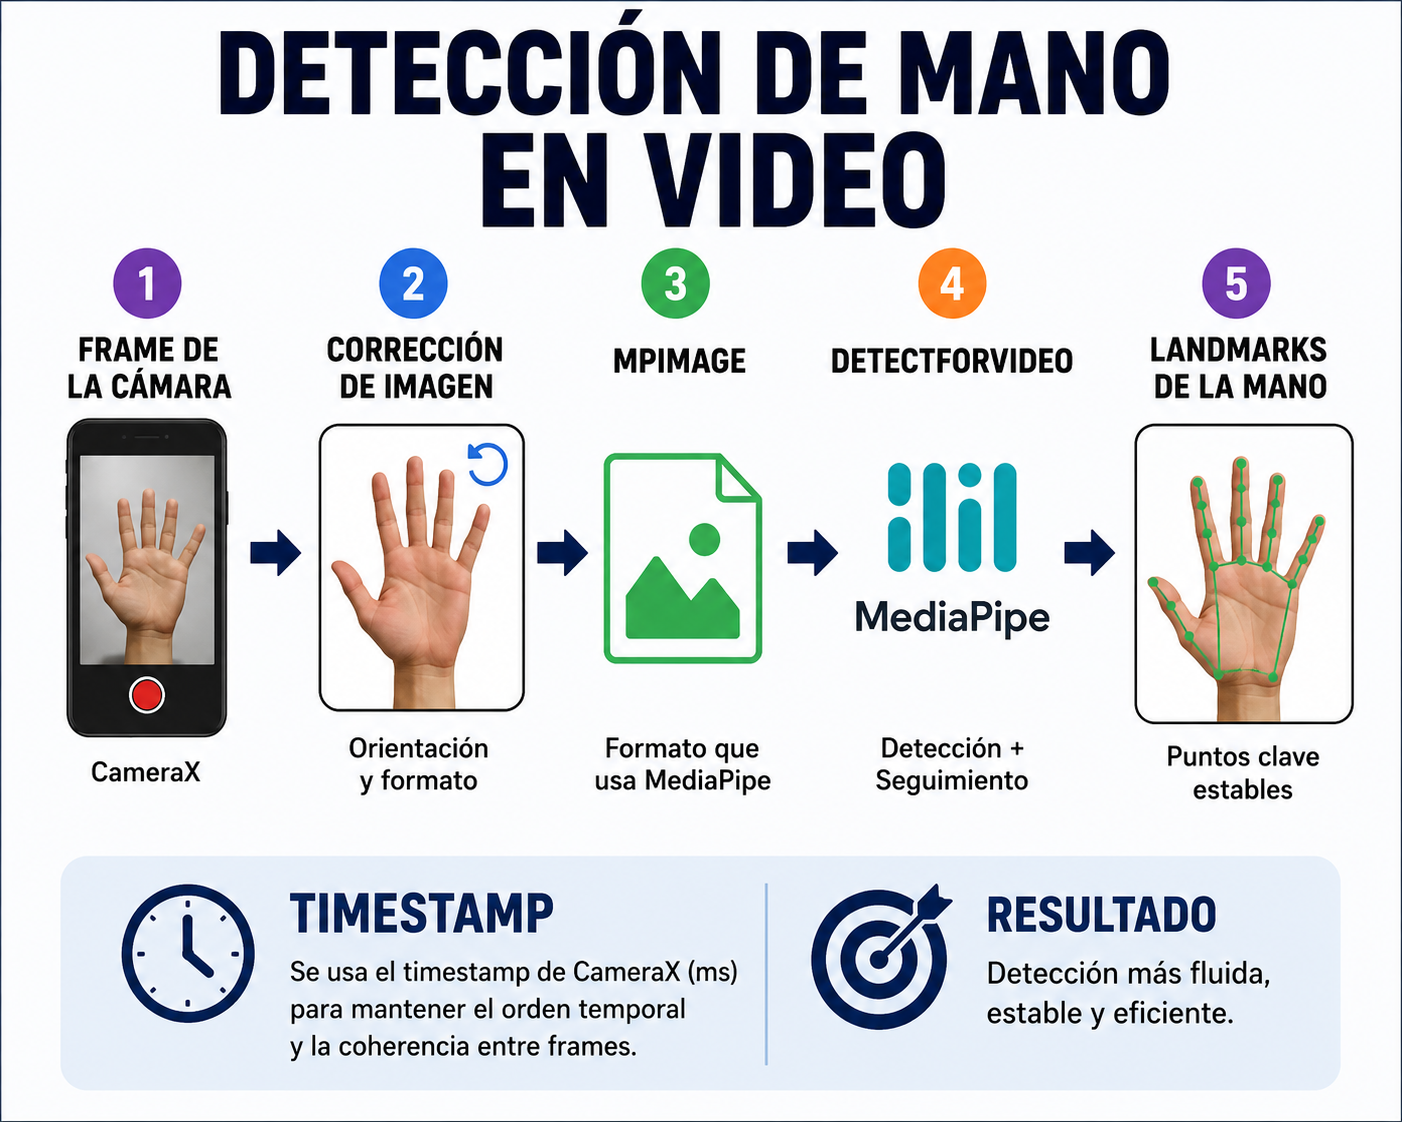
\includegraphics[width=0.6\textwidth]{images/deteccionMano.png}
		\caption{Flujo de detección de la mano en video mediante CameraX y MediaPipe.}
		\label{fig:deteccion-mano-video}
	\end{figure}
	
	Esta etapa funciona como el puente entre la captura visual de la cámara y la inferencia realizada por el sistema de reconocimiento.
	
	\subsubsection{Impacto de las variantes de normalización}
	
	
	Para la integración del modelo de clasificación en la aplicación móvil se identificó que la normalización de los landmarks no era un detalle menor del preprocesamiento, sino un factor determinante para la estabilidad del reconocimiento. Aunque MediaPipe entrega coordenadas relativas al tamaño de la imagen, dichas coordenadas aún conservan variaciones asociadas a la posición, escala y orientación de la mano dentro del encuadre, así como diferencias derivadas del entorno donde se generan los landmarks.
	
	Dada esta situación en las pruebas se evaluaron distintas variantes de normalización con la finalidad de mantener congruencia entre el entrenamiento realizado en computadora y la inferencia ejecutada posteriormente en Android. El problema principal era que pequeñas diferencias entre la representación utilizada en el entrenamiento y la representación generada en el dispositivo móvil podían provocar cambios importantes en la clasificación. En otras palabras, aunque el modelo fuera el mismo, si el vector de entrada se construía de forma distinta, el comportamiento del sistema también cambiaba.
	
	La primera variante utilizada consistía en restar a cada coordenada el valor mínimo correspondiente de su eje. Bajo este enfoque, las coordenadas se trasladaban hacia un origen local definido por la esquina superior izquierda de la mano detectada. Esta estrategia reducía la dependencia respecto a la posición absoluta de la mano dentro de la imagen, ya que el modelo no recibía directamente dónde se encontraba la mano en el encuadre, sino la distribución relativa de sus puntos clave.
	
	\[
	x_i' = x_i - \min(x), \qquad y_i' = y_i - \min(y)
	\]
	
	Aunque esta variante permitió obtener resultados funcionales en las primeras pruebas, todavía conservaba dependencia respecto al tamaño aparente de la mano. Por ejemplo, una misma seña realizada cerca de la cámara generaba valores de mayor magnitud que la misma seña realizada a mayor distancia. Esta diferencia podía afectar la estabilidad del modelo, específicamente al pasar de pruebas en computadora a pruebas en dispositivo móvil.
	
	\begin{figure}[H]
		\centering
		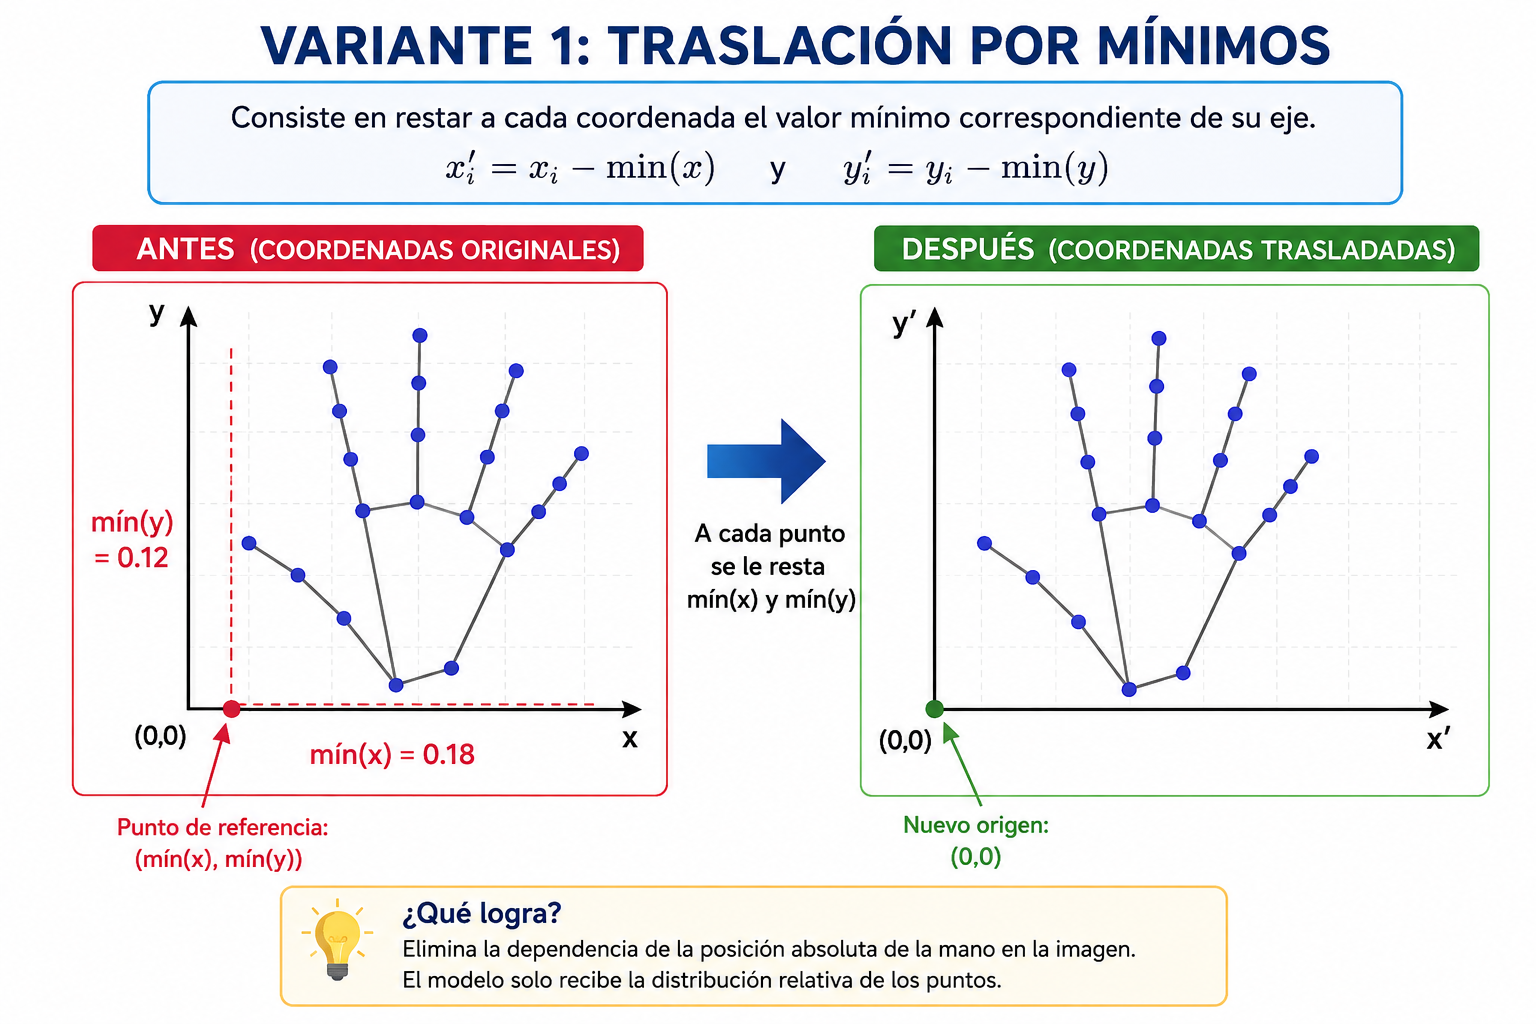
\includegraphics[width=0.9\textwidth]{images/va1.png}
		\caption{Variante 1.}
		\label{fig:Variante1}
	\end{figure}
	
	Posteriormente se evaluó una normalización basada en una escala única, calculada a partir del mayor valor entre el ancho y el alto de la mano detectada. Esta variante buscaba conservar la proporción geométrica general de la mano y evitar deformaciones independientes entre los ejes.
	
	\[
	s = \max(w,h)
	\]
	
	\[
	x_i' = \frac{x_i - \min(x)}{s}, \qquad y_i' = \frac{y_i - \min(y)}{s}
	\]
	
	Pero se observó que esta estrategia podía ser sensible a cambios de orientación y a variaciones en la forma en que la mano ocupaba el encuadre. Al utilizar una sola escala para ambos ejes, ciertos cambios en la proporción visible de la mano podían alterar la geometría relativa de los landmarks respecto a la distribución aprendida en el entrenamiento. Esto era perceptible al comparar el comportamiento entre laptop y dispositivo móvil asi como en orientación vertical.
	
	\begin{figure}[H]
		\centering
		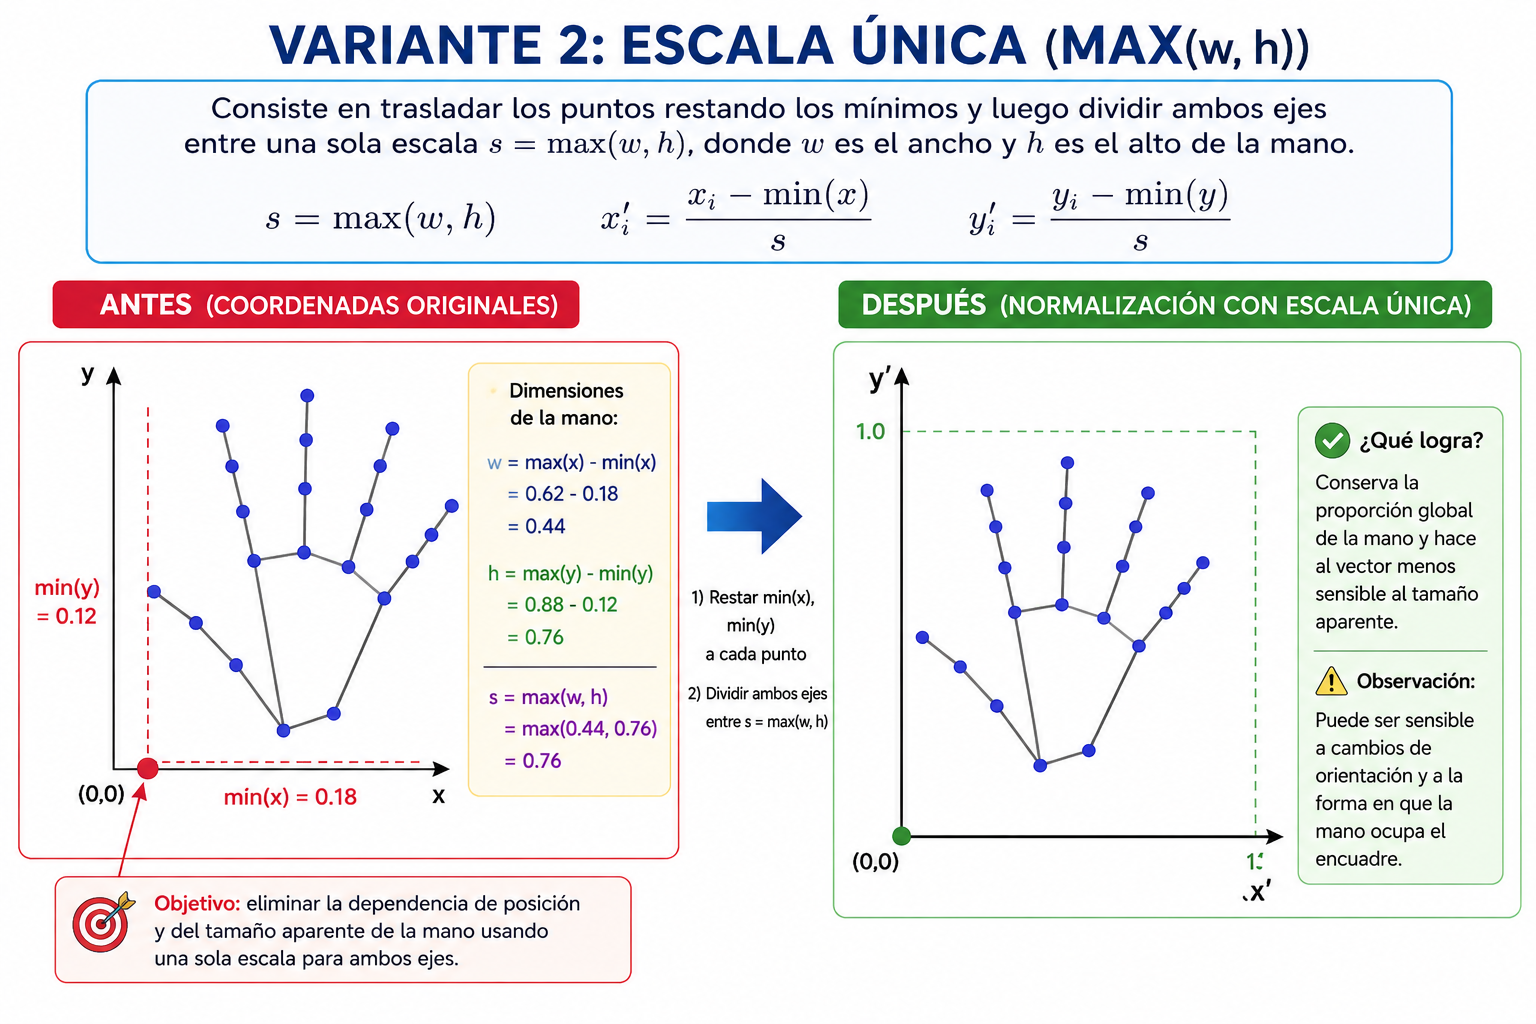
\includegraphics[width=0.9\textwidth]{images/va2.png}
		\caption{Variante 2.}
		\label{fig:Variante1}
	\end{figure}
	
	La variante final adoptada consistió en normalizar cada eje de manera independiente, utilizando el ancho de la mano para las coordenadas \(x\) y el alto de la mano para las coordenadas \(y\). Esta estrategia fue la que presentó mayor consistencia entre el entrenamiento y la inferencia móvil en las pruebas experimentales realizadas, además de proporcionar mayor estabilidad general en el reconocimiento continuo de señas.
	
	\[
	w = \max(x) - \min(x), \qquad h = \max(y) - \min(y)
	\]
	
	\[
	x_i' = \frac{x_i - \min(x)}{w}, \qquad y_i' = \frac{y_i - \min(y)}{h}
	\]
	
	Esta normalización fue incorporada tanto en el entrenamiento final del modelo como en la implementación móvil del analizador. En el entrenamiento, cada muestra del dataset fue procesada separando las coordenadas \(x\) y \(y\), calculando el ancho y alto de la mano y reensamblando posteriormente el vector en el formato \([x_0,y_0,x_1,y_1,\ldots,x_{20},y_{20}]\). Tambien en Android el método encargado de extraer características construye un arreglo de 42 valores bajo la misma lógica, permitiendo mantener consistencia entre el entorno de entrenamiento y la inferencia ejecutada en el dispositivo móvil.
	
	\begin{figure}[H]
		\centering
		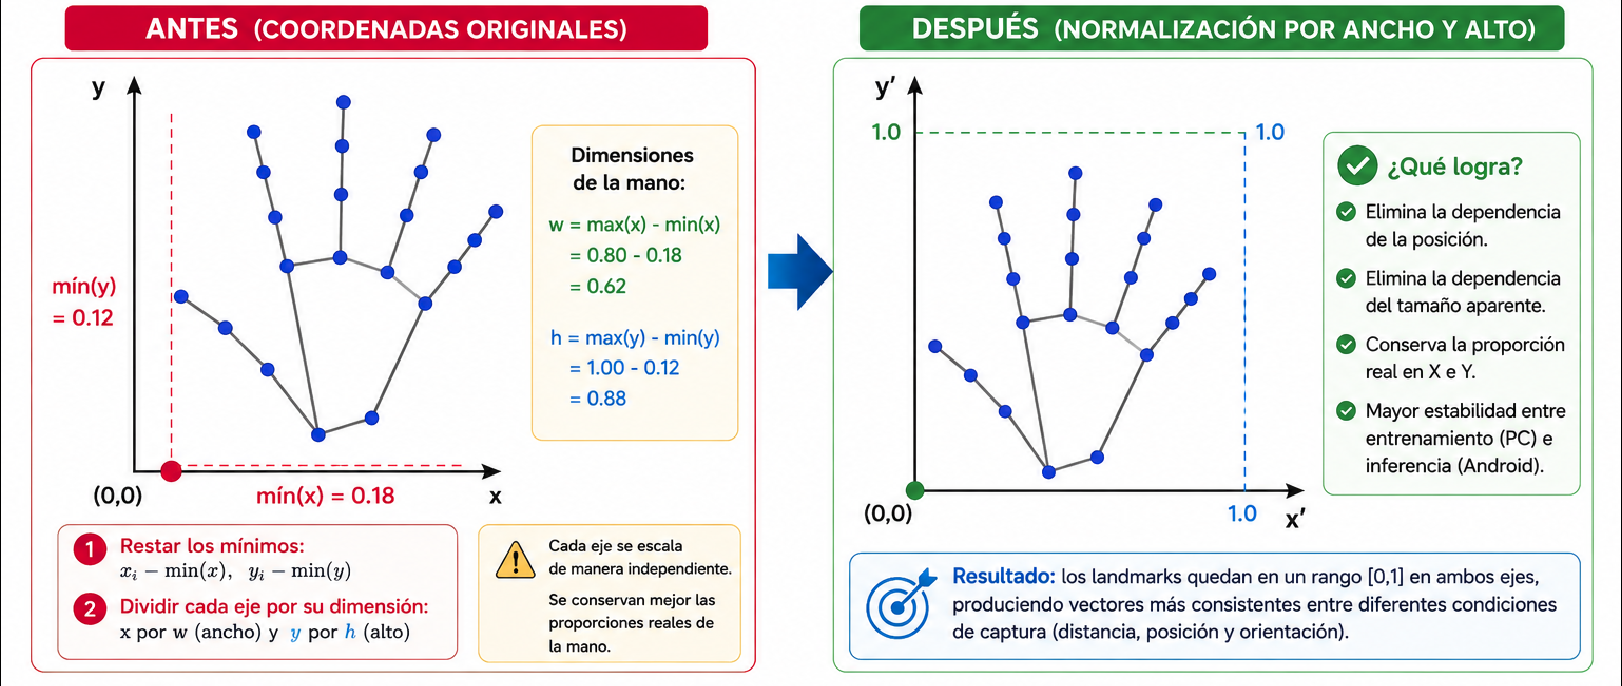
\includegraphics[width=1\textwidth]{images/va3.png}
		\caption{Variante 3.}
		\label{fig:Variante1}
	\end{figure}
	{
		\rowcolors{2}{rowblue}{white}
		
		\small
		\renewcommand{\arraystretch}{1.2}
		
		\begin{table}[H]
			\centering
			\caption{Comparación de variantes de normalización evaluadas.}
			\label{tab:normalizacion_landmarks}
			
			\begin{tabularx}{\textwidth}{
					!{\vrule width 0.6pt}
					>{\centering\arraybackslash}p{3.0cm}
					!{\vrule width 0.6pt}
					>{\centering\arraybackslash}p{3.7cm}
					!{\vrule width 0.6pt}
					>{\centering\arraybackslash}X
					!{\vrule width 0.6pt}
				}
				\hline
				\rowcolor{headerblue}
				\textcolor{white}{\textbf{Variante}} &
				\textcolor{white}{\textbf{Descripción}} &
				\textcolor{white}{\textbf{Observación en las pruebas}} \\
				\hline
				
				Traslación por mínimos &
				Resta \(\min(x)\) y \(\min(y)\) a cada coordenada. &
				Reduce la dependencia respecto a la posición, pero conserva variaciones asociadas al tamaño aparente de la mano. \\
				\hline
				
				Escala única &
				Divide ambos ejes entre \(\max(w,h)\). &
				Conserva proporción global, pero puede ser sensible a orientación, encuadre y diferencias entre laptop y móvil. \\
				\hline
				
				Normalización por ancho y alto &
				Divide \(x\) entre \(w\) y \(y\) entre \(h\). &
				Fue la variante final debido a su mejor estabilidad general y mejor correspondencia entre entrenamiento e inferencia móvil. \\
				\hline
				
			\end{tabularx}
		\end{table}
	}
	Esta última variante también permitió reducir la redundancia entre los scripts de prueba en computadora y la implementación móvil. En el desarrollo existían diferencias entre algunas pruebas realizadas en laptop y el comportamiento observado en Android, principalmente porque no siempre se construía el vector de características exactamente bajo la misma lógica. Al unificar el procedimiento de normalización, el modelo recibió una representación más consistente en ambos entornos.
	
	La normalización final no solo funcionó como una etapa matemática de preprocesamiento, sino como un mecanismo de alineación entre el entorno experimental y el entorno móvil. Esta decisión permitió mejorar la estabilidad de los landmarks utilizados por el clasificador y reducir errores derivados de cambios en distancia, posición y escala de la mano dentro del encuadre.
	
	\paragraph{Diferencias entre MediaPipe de escritorio y Android}
	
	Durante las pruebas preliminares de inferencia se observó que los vectores de características generados en Android y en entorno de escritorio no eran completamente idénticos, incluso utilizando el mismo modelo, la misma estrategia de normalización y un pipeline equivalente de extracción basado en MediaPipe Hands.
	
	Para analizar este funcionamiento se realizaron capturas de landmarks normalizados tanto en la aplicación Android como en los scripts de inferencia ejecutados en computadora. Las pruebas se realizaron utilizando las vocales \texttt{A}, \texttt{E}, \texttt{I}, \texttt{O} y \texttt{U}. Los resultados mostraron que, aunque la geometría general de la mano permanecía visualmente similar, existían diferencias numéricas entre coordenadas equivalentes.
	
	La Tabla 35 muestra una comparación parcial entre algunos valores normalizados obtenidos en Android y en escritorio para las distintas vocales evaluadas.
	{
		\rowcolors{2}{rowblue}{white}
		
		\scriptsize
		\renewcommand{\arraystretch}{0.92}
		
		\begin{table}[H]
			\centering
			\caption{Comparación parcial de landmarks normalizados entre Android y escritorio}
			\label{tab:comparacion_android_pc_landmarks}
			
			\resizebox{0.68\textwidth}{!}{
				
				\begin{tabular}{
						!{\vrule width 0.4pt}
						c
						!{\vrule width 0.4pt}
						c
						!{\vrule width 0.4pt}
						c
						!{\vrule width 0.4pt}
						c
						!{\vrule width 0.4pt}
					}
					
					\hline
					
					\rowcolor{headerblue}
					\textcolor{white}{\textbf{Seña}} &
					\textcolor{white}{\textbf{Coord.}} &
					\textcolor{white}{\textbf{Android}} &
					\textcolor{white}{\textbf{PC}} \\
					
					\hline
					
					A & $x_0$ & 0.998487 & 0.913442 \\
					A & $y_0$ & 0.794394 & 0.214582 \\
					A & $x_1$ & 1.000000 & 0.587214 \\
					A & $y_1$ & 0.489702 & 0.664238 \\
					A & $x_2$ & 0.855234 & 0.421553 \\
					A & $y_2$ & 0.284667 & 0.731882 \\
					\hline
					
					E & $x_0$ & 0.999735 & 0.948215 \\
					E & $y_0$ & 0.926312 & 0.332104 \\
					E & $x_1$ & 0.952348 & 0.621478 \\
					E & $y_1$ & 0.534341 & 0.702183 \\
					E & $x_2$ & 1.000000 & 0.482771 \\
					E & $y_2$ & 0.190050 & 0.755621 \\
					\hline
					
					I & $x_0$ & 0.999992 & 0.964802 \\
					I & $y_0$ & 1.000000 & 0.276511 \\
					I & $x_1$ & 1.000000 & 0.598773 \\
					I & $y_1$ & 0.410600 & 0.655104 \\
					I & $x_2$ & 0.978261 & 0.503442 \\
					I & $y_2$ & 0.138881 & 0.784221 \\
					\hline
					
					O & $x_0$ & 0.960401 & 0.882416 \\
					O & $y_0$ & 1.000000 & 0.301882 \\
					O & $x_1$ & 1.000000 & 0.564290 \\
					O & $y_1$ & 0.483938 & 0.618114 \\
					O & $x_2$ & 0.860486 & 0.493782 \\
					O & $y_2$ & 0.245422 & 0.701554 \\
					\hline
					
					U & $x_0$ & 0.710005 & 0.877531 \\
					U & $y_0$ & 0.649558 & 0.161583 \\
					U & $x_1$ & 1.000000 & 0.556965 \\
					U & $y_1$ & 0.250080 & 0.605672 \\
					U & $x_2$ & 0.906684 & 1.000000 \\
					U & $y_2$ & 0.040404 & 0.257961 \\
					\hline
					
				\end{tabular}
				
			}
		\end{table}
	}
	
	
	Aunque las diferencias observadas pueden parecer pequeñas desde el punto de vista numérico, en modelos de clasificación basados en landmarks representan variaciones geométricas relevantes dentro del espacio de características utilizado durante el entrenamiento. Esto puede modificar parcialmente la distribución espacial esperada por el modelo y afectar la estabilidad de la inferencia.
	
	Se identificó que estas variaciones probablemente se encuentran relacionadas con múltiples factores presentes entre ambos entornos de ejecución, entre ellos:
	
	\begin{itemize}
		\item Diferencias internas entre la implementación móvil y de escritorio de MediaPipe Hands.
		\item Uso de cámaras distintas y resoluciones diferentes.
		\item Rotación automática de imágenes en Android.
		\item Efectos de espejo horizontal en cámara frontal.
		\item Diferencias de aspect ratio y escalado de imagen.
		\item Variaciones en el tracking temporal de landmarks.
		\item Diferencias en el preprocesamiento interno realizado por cada plataforma.
	\end{itemize}
	
	Algunas señas presentaban un comportamiento más estable en escritorio que en Android, particularmente en configuraciones donde la orientación del dispositivo cambiaba constantemente o existían ligeras variaciones en el encuadre de la mano. Esto mostró que mantener exactamente el mismo pipeline de extracción y normalización entre entrenamiento e inferencia resulta fundamental para conservar la estabilidad del sistema.
	
	\subsubsection{Sensibilidad ante orientación e iluminación}
	
	\begin{figure}[H]
		\centering
		
		\begin{subfigure}[b]{0.32\textwidth}
			\centering
			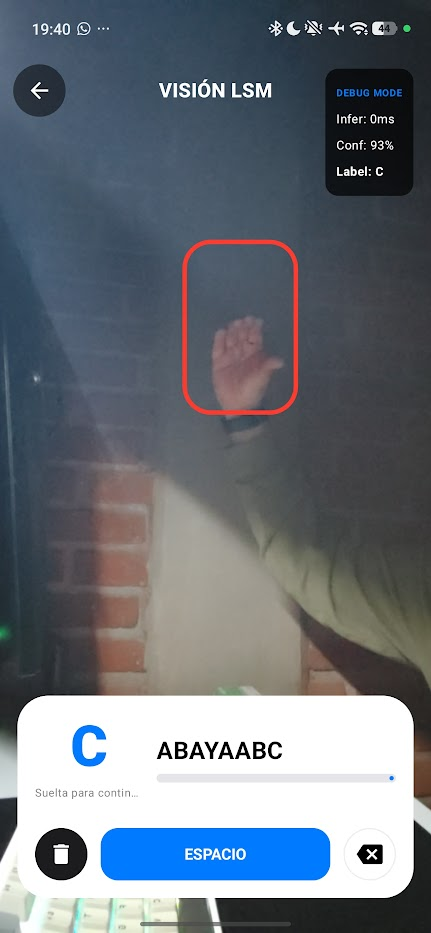
\includegraphics[width=\linewidth]{images/fig55_1.jpg}
			\caption{}
		\end{subfigure}
		\hfill
		\begin{subfigure}[b]{0.32\textwidth}
			\centering
			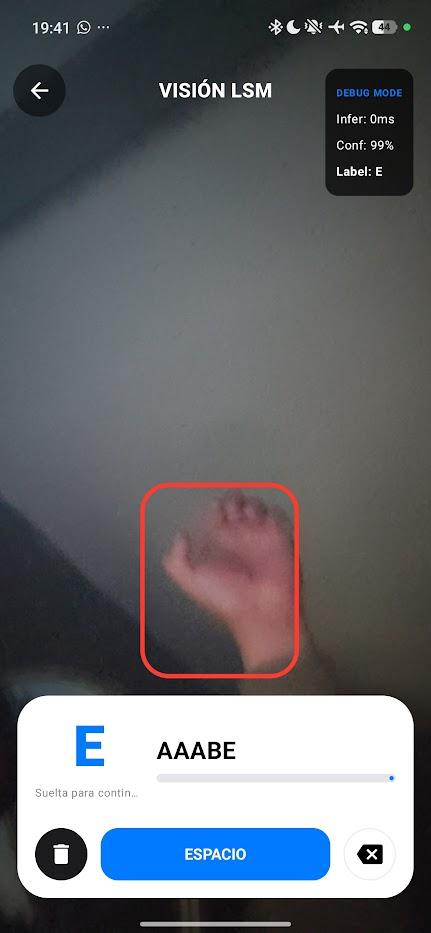
\includegraphics[width=\linewidth]{images/fig55_2.jpg}
			\caption{}
		\end{subfigure}
		\hfill
		\begin{subfigure}[b]{0.32\textwidth}
			\centering
			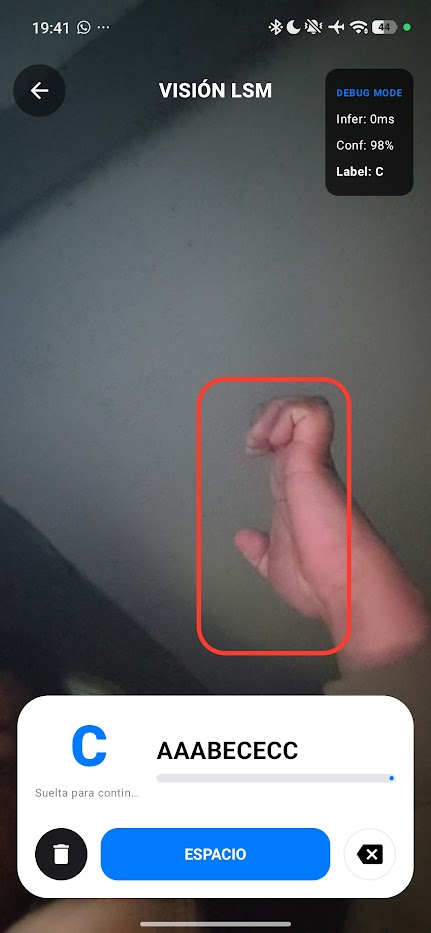
\includegraphics[width=\linewidth]{images/fig55_3.jpg}
			\caption{}
		\end{subfigure}
		
		\caption{Pruebas realizadas bajo condiciones complejas de captura. 
			(a) Reconocimiento correcto bajo baja iluminación y una distancia aproximada de 1.5 metros, superior a la considerada inicialmente en las pruebas base. 
			(b) Detección estable bajo una orientación extrema del dispositivo móvil, incluso con perspectiva inclinada y condiciones visuales mejorables. 
			(c) Error de clasificación provocado por una rotación pronunciada de la mano sobre su propio eje, generando una geometría similar a la letra ``C'' desde la perspectiva del modelo.}
		
		\label{fig:pruebas_condiciones_complejas}
	\end{figure}
	
	En estas pruebas se evaluó el comportamiento del sistema bajo condiciones complejas de captura, incluyendo escenarios con baja iluminación, variaciones extremas de orientación y rotaciones pronunciadas de la mano.
	
	En la Figura~\ref{fig:pruebas_condiciones_complejas}(a) se observa una prueba realizada bajo iluminación deficiente y a una distancia aproximada de 1.5 metros, superior a la considerada inicialmente en las pruebas base del sistema. A pesar de la pérdida considerable de detalle visual y del ruido presente en la imagen, el sistema logró mantener la detección de la mano y realizar correctamente la clasificación de la seña.
	
	La Figura~\ref{fig:pruebas_condiciones_complejas}(b) muestra una prueba realizada con el dispositivo móvil en una orientación extrema, introduciendo cambios importantes en la perspectiva y geometría de captura. Aunque estas condiciones generan deformaciones espaciales adicionales sobre la mano detectada, el sistema logró conservar un comportamiento funcional y mantener la clasificación correcta de la seña aunque baja unos puntos la confianza.
	
	La Figura~\ref{fig:pruebas_condiciones_complejas}(c) se presenta uno de los errores observados en las pruebas. En este caso, la mano fue rotada sobre su propio eje, provocando que la geometría resultante de los landmarks adquiriera una forma visualmente similar a la letra ``C''. Es así que el sistema realizó una clasificación incorrecta. Este rendimiento muestra  que ciertas rotaciones extremas pueden modificar significativamente la distribución espacial de los landmarks y generar ambigüedad entre algunas clases.
	
	
	\begin{figure}[H]
		\centering
		
		\begin{subfigure}[b]{0.32\textwidth}
			\centering
			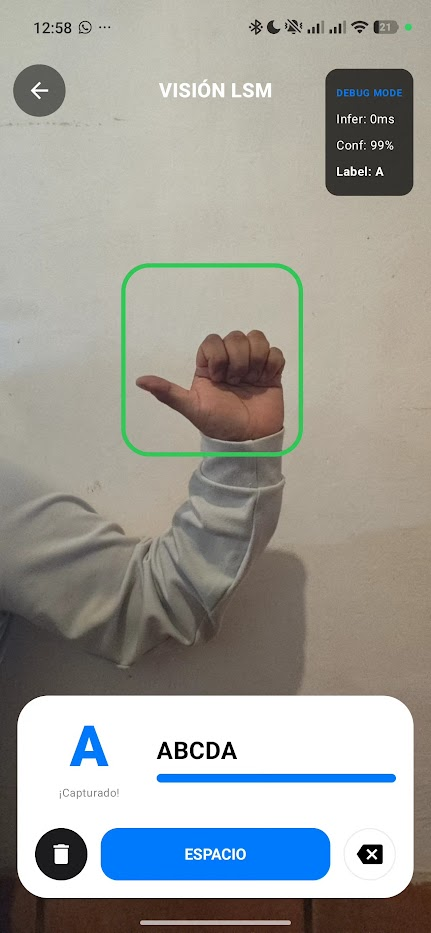
\includegraphics[width=\linewidth]{images/A1.png}
			\caption{}
		\end{subfigure}
		\hfill
		\begin{subfigure}[b]{0.32\textwidth}
			\centering
			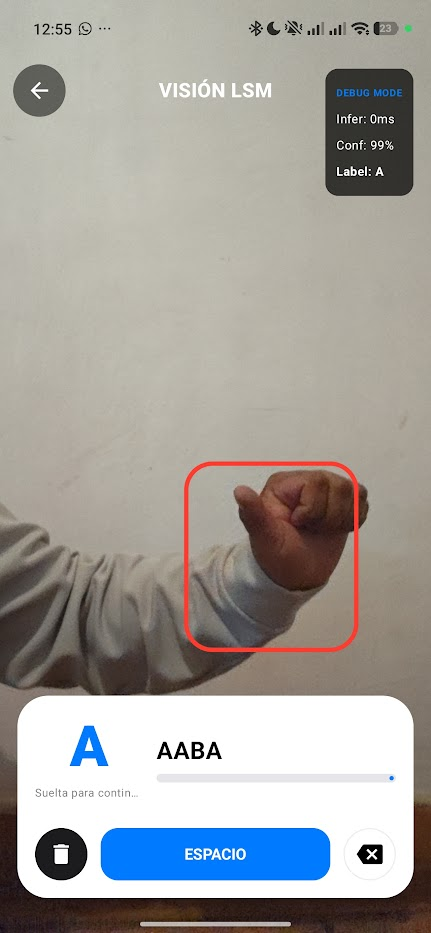
\includegraphics[width=\linewidth]{images/A2.png}
			\caption{}
		\end{subfigure}
		\hfill
		\begin{subfigure}[b]{0.32\textwidth}
			\centering
			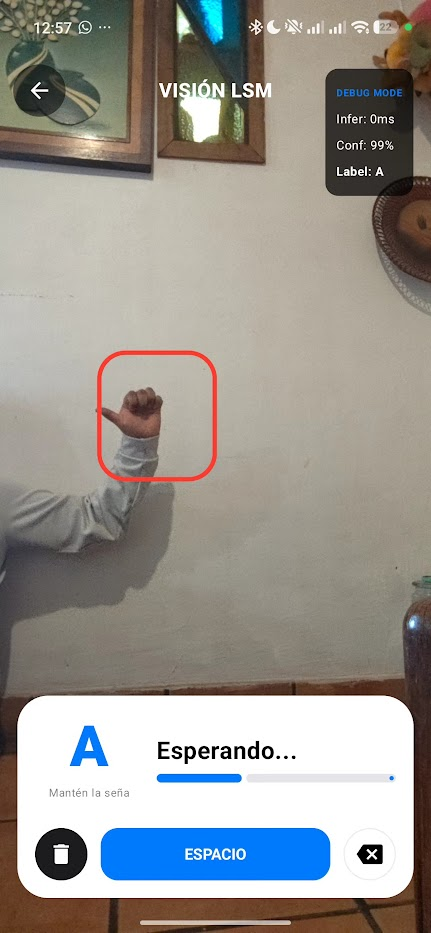
\includegraphics[width=\linewidth]{images/A3.png}
			\caption{}
		\end{subfigure}
		
		\caption{Pruebas realizadas a distintas distancias de captura. 
			(a) Distancia corta con alta estabilidad geométrica de landmarks. 
			(b) Distancia media dentro del rango de operación recomendado para el sistema. 
			(c) Distancia aproximada de 1.3 metros, donde el sistema aún mantiene detección y clasificación funcional, aunque con menor estabilidad temporal debido a la reducción del tamaño aparente de la mano.}
		
		\label{fig:pruebas_distancia}
	\end{figure}
	
	En estas pruebas se observó que el sistema mantiene un comportamiento estable cuando la mano se encuentra dentro de un rango de captura aproximado entre 30 cm y 1.3 metros respecto a la cámara del dispositivo móvil. Dentro de este intervalo, MediaPipe Hands logró conservar una detección consistente de landmarks y el modelo mantuvo clasificaciones funcionalmente correctas en la mayoría de escenarios evaluados.
	
	Como puede observarse en la Figura~\ref{fig:pruebas_distancia}, al incrementar progresivamente la distancia respecto a la cámara, la mano ocupa una menor proporción del frame y se reduce la cantidad de detalle visual disponible para el sistema. A pesar de esto el prototipo logró conservar detección y clasificación incluso bajo distancias superiores a las inicialmente consideradas en las pruebas base.
	
	También se observó que distancias mayores pueden introducir ligeras variaciones en la estabilidad temporal de la inferencia, principalmente debido a la reducción espacial de los landmarks detectados y al aumento de sensibilidad frente a pequeñas variaciones geométricas de la mano.
	
	Se tiene que considerar que el sistema fue diseñado para reconocer señas realizadas bajo condiciones razonables de captura y ejecución. Es por eso que la aplicación incorpora un área guía de posicionamiento que ayuda al usuario a mantener una escala, orientación y distancia relativamente consistentes en el reconocimiento.
	
	La forma en que reacciona el sistema a mayores distancias se encuentra relacionado con el proceso de normalización utilizado en la extracción de características y con la propia arquitectura interna de MediaPipe Hands.
	
	Debido a que el modelo trabaja con coordenadas relativas normalizadas y no con posiciones absolutas en pantalla, la geometría general de la mano puede conservarse incluso cuando su tamaño aparente disminuye dentro del frame capturado. Así es como las señas realizadas a distintas distancias pueden seguir produciendo distribuciones espaciales similares dentro del vector de características utilizado en la inferencia.
	
	MediaPipe Hands implementa internamente un proceso de detección de región de interés (ROI), donde la mano detectada es localizada, recortada y reescalada antes de realizar la estimación de landmarks. Esto permite mantener una representación relativamente consistente de la mano aun cuando ésta ocupe una región pequeña dentro de la imagen original.
	
	Al final el sistema logró conservar detección y clasificación de señas incluso a distancias superiores a las consideradas inicialmente en las pruebas base. Sin embargo, al aumentar excesivamente la distancia también disminuye la cantidad de información visual disponible, provocando menor estabilidad temporal y mayor sensibilidad ante pequeñas variaciones geométricas.
	
	\subsection{Integración del modelo TensorFlow Lite}
	
	Una vez termianda la etapa de entrenamiento y validación del clasificador basado en landmarks, el siguiente paso consistió en integrar el modelo dentro de la aplicación Android para ejecutar el modelo de clasificación local  en el dispositivo móvil. Para ello se utilizó TensorFlow Lite, una versión optimizada de TensorFlow diseñada específicamente para entornos embebidos y dispositivos con recursos limitados.
	
	La integración del modelo se realizó mediante la clase \texttt{Interpreter} de TensorFlow Lite, encargada de cargar el archivo \texttt{.tflite} y ejecutar inferencias utilizando tensores de entrada y salida definidos previamente en la conversión del modelo.
	
	\begin{lstlisting}[language=Java]
		val options = Interpreter.Options().apply {
			setNumThreads(4)
			setUseNNAPI(true)
		}
		
		interpreter = Interpreter(
		FileUtil.loadMappedFile(context, modelAssetPath),
		options
		)
	\end{lstlisting}
	
	Al iniciar el interprete se habilita el uso de múltiples hilos de ejecución mediante \texttt{setNumThreads(4)} con el objetivo de mejorar la latencia de inferencia en dispositivos móviles. Tambien se activa la aceleración mediante NNAPI utilizando \texttt{setUseNNAPI(true)}, permitiendo que Android delegue ciertas operaciones a aceleradores de hardware compatibles cuando se encuentran disponibles.
	
	El modelo final recibe como entrada un vector de 42 valores correspondientes a las coordenadas normalizadas de los 21 landmarks de la mano detectada. Cada landmark aporta una coordenada \(x\) y una coordenada \(y\), organizadas en el siguiente formato:
	
	\[
	[x_0,y_0,x_1,y_1,\ldots,x_{20},y_{20}]
	\]
	
	Antes de ejecutar la clasificación la aplicación valida que el vector tenga exactamente 42 características para garantizar compatibilidad con la estructura utilizada en el entrenamiento.
	
	\begin{lstlisting}[language=Java]
		if (features42.size != 42) {
			return ClassificationResult("?", 0f)
		}
	\end{lstlisting}
	
	Luego el vector es copiado hacia un tensor de entrada de tipo \texttt{Float32}, manteniendo la misma representación utilizada en el entrenamiento del modelo.
	
	\begin{lstlisting}[language=Java]
		val input = Array(1) { FloatArray(42) }
		System.arraycopy(features42, 0, input[0], 0, 42)
	\end{lstlisting}
	
	La salida del modelo consiste en un arreglo de probabilidades, donde cada posición representa la confianza asociada a una clase del alfabeto LSM evaluado. Después de ejecutar la inferencia, la aplicación recorre el tensor de salida para localizar la clase con mayor puntuación.
	
	\begin{lstlisting}[language=Java]
		localInterpreter.run(input, output)
		
		var bestIndex = 0
		var bestScore = -1f
		
		for (i in output[0].indices) {
			if (output[0][i] > bestScore) {
				bestScore = output[0][i]
				bestIndex = i
			}
		}
	\end{lstlisting}
	
	La clase seleccionada corresponde al índice con mayor probabilidad dentro del vector de salida. Dicho valor es utilizado tanto para mostrar la predicción en pantalla como para estimar el nivel de confianza asociado al reconocimiento.
	
	Aunque internamente el modelo produce valores asociados a cada clase, el proceso de selección final equivale conceptualmente a aplicar una función de activación tipo Softmax, donde la categoría con mayor puntuación es interpretada como la predicción dominante. En consecuencia, el sistema obtiene simultáneamente una etiqueta de clasificación y un valor de confianza normalizado entre 0 y 1.
	
	La inferencia se ejecuta completamente de manera local dentro del dispositivo móvil, evitando depender de servidores externos o conexión a internet. Esto permite reducir latencia, mejorar privacidad y mantener disponibilidad del sistema incluso en entornos sin conectividad. Además, al trabajar únicamente con landmarks y no con imágenes completas, el tamaño del vector de entrada se reduce considerablemente, permitiendo que el modelo ejecute inferencias continuas con un costo computacional relativamente bajo.
	
	\subsection{Optimización para dispositivos móviles}
	
	La integración del modelo dentro de una aplicación móvil requirió considerar restricciones distintas a las presentes en el entrenamiento en computadora. En un dispositivo móvil, el sistema debe operar con recursos limitados de procesamiento, memoria y energía, además de compartir dichos recursos con la cámara, la interfaz gráfica, el sistema operativo y otros procesos internos de Android.
	
	Por esta razón, la optimización del prototipo no se abordó únicamente desde el tamaño del modelo, sino desde el diseño completo del flujo de inferencia. La decisión principal consistió en evitar el procesamiento directo de imágenes completas y utilizar una representación basada en landmarks de la mano. De esta forma, la aplicación no envía al clasificador una imagen RGB, sino un vector numérico reducido que describe la geometría de la seña.
	
	\subsubsection{Tamaño del modelo}
	
	El modelo final utilizado en la aplicación fue exportado al formato \texttt{.tflite}, lo que permitió integrarlo directamente dentro de los recursos locales de Android. El archivo \texttt{model\_lsm\_v3.tflite} tiene un tamaño aproximado de 68.6 kB, mientras que el archivo de etiquetas \texttt{labels.txt} ocupa únicamente 42 bytes. Estos tamaños permiten que el modelo y sus clases asociadas sean incluidos dentro de la carpeta \texttt{assets} de la aplicación sin representar una carga significativa para el almacenamiento del dispositivo.
	
	En el desarrollo también se generaron versiones previas del modelo, como \texttt{model\_lsmv2.tflite} y \texttt{model\_lsmv2.1.tflite}, con un tamaño aproximado de 24.2 kB. Sin embargo, la versión \texttt{model\_lsm\_v3.tflite}, aunque ligeramente mayor, fue la seleccionada para la integración final debido a que presentó un mejor comportamiento general en las pruebas de reconocimiento.
	
	{
		\rowcolors{2}{rowblue}{white}
		
		\small
		\renewcommand{\arraystretch}{1.15}
		
		\begin{table}[H]
			\centering
			\caption{Tamaño de los recursos utilizados para la inferencia móvil.}
			\label{tab:tamanio_recursos_tflite}
			
			\begin{tabular}{
					!{\vrule width 0.6pt}
					>{\centering\arraybackslash}p{5.5cm}
					!{\vrule width 0.6pt}
					>{\centering\arraybackslash}p{4.0cm}
					!{\vrule width 0.6pt}
				}
				
				\hline
				
				\rowcolor{headerblue}
				\textcolor{white}{\textbf{Recurso}} &
				\textcolor{white}{\textbf{Tamaño aproximado}} \\
				
				\hline
				
				\texttt{model\_lsmv2.tflite} &
				24.2 kB \\
				\hline
				
				\texttt{model\_lsmv2.1.tflite} &
				24.2 kB \\
				\hline
				
				\texttt{model\_lsm\_v3.tflite} &
				68.6 kB \\
				\hline
				
				\texttt{model\_lsm\_v3.1.tflite} &
				68.6 kB \\
				\hline
				
				\texttt{labels.txt} &
				42 bytes \\
				\hline
				
			\end{tabular}
		\end{table}
	}
	
	El tamaño reducido del modelo se debe principalmente a que el clasificador no fue entrenado para procesar imágenes completas, sino vectores de características derivados de los landmarks. Esto permitió obtener un modelo mucho más ligero que una arquitectura convolucional basada en imágenes, lo cual favorece su ejecución en dispositivos móviles.
	
	\subsubsection{Inferencia local}
	

	
	Ejecutar el modelo de forma local resulta importante por tres razones principales. Primero, reduce la dependencia de la conectividad, ya que la aplicación puede operar aun cuando el dispositivo no tenga acceso a red. Segundo, disminuye el tiempo asociado al envío y recepción de datos hacia un servidor remoto. Tercero, favorece la privacidad del usuario, debido a que los frames capturados por la cámara no necesitan ser transmitidos fuera del dispositivo.
	
	El modelo se carga desde los assets de la aplicación mediante \texttt{FileUtil.loadMappedFile}, y posteriormente se ejecuta usando la clase \texttt{Interpreter} de TensorFlow Lite.
	
	\begin{lstlisting}[language=Java]
		interpreter = Interpreter(
		FileUtil.loadMappedFile(context, modelAssetPath),
		options
		)
	\end{lstlisting}
	
	Así es como el archivo \texttt{.tflite} queda disponible localmente para recibir el vector de entrada y producir una predicción sin intervención de servicios externos.
	
	\subsubsection{Reducción del costo computacional mediante landmarks}
	
	Una de las decisiones más importantes para optimizar el prototipo fue utilizar landmarks de la mano como entrada del modelo en lugar de imágenes completas. El detector de MediaPipe obtiene 21 puntos clave de la mano, y de cada punto se utilizan únicamente sus coordenadas \(x\) y \(y\). Como resultado, cada frame válido se transforma en un vector de 42 valores numéricos como se ha revisado en anteriores secciones.
	
	Esta representación reduce de forma significativa la cantidad de información procesada por el clasificador. En lugar de analizar todos los píxeles de una imagen, el modelo recibe únicamente una descripción geométrica de la mano. Esto disminuye el número de operaciones necesarias en la clasificación y permite que el modelo sea más adecuado para ejecutarse en dispositivos móviles.
	
	En el analizador de la aplicación, esta transformación se realiza después de que MediaPipe detecta una mano válida. El método encargado de extraer características construye un arreglo de 42 valores normalizados, manteniendo la misma lógica utilizada en el entrenamiento.
	
	\begin{lstlisting}[language=Java]
		val f = FloatArray(42)
		
		for (i in 0 until 21) {
			f[i * 2] = (xList[i] - minX) / safeW
			f[i * 2 + 1] = (yList[i] - minY) / safeH
		}
	\end{lstlisting}
	
	Esta decisión también permitió separar dos tareas distintas dentro del sistema. MediaPipe se encarga de detectar la mano y estimar sus puntos clave, mientras que el modelo TensorFlow Lite únicamente clasifica la configuración geométrica representada por esos puntos. Esta separación reduce la complejidad del modelo de clasificación y facilita su ejecución local.
	
	
	\subsubsection{Uso de NNAPI, multihilo y procesamiento concurrente}
	
	Para mejorar el desempeño del modelo en Android, la integración de TensorFlow Lite no se realizó únicamente cargando el archivo \texttt{.tflite}, sino configurando el intérprete con opciones específicas para ejecución móvil. En la clase \texttt{LsmClassifier}, el modelo se inicializa mediante la clase \texttt{Interpreter}, utilizando el archivo \texttt{model\_lsm\_v3.tflite} almacenado dentro de los assets de la aplicación.
	
	El uso de \texttt{setNumThreads(4)} se incorporó debido a que la aplicación no ejecuta una sola tarea aislada, sino varias operaciones simultáneas: la cámara captura frames de manera continua, CameraX entrega dichos frames al analizador, MediaPipe procesa la imagen para detectar la mano, el analizador construye el vector de características y TensorFlow Lite ejecuta la clasificación. Además, la interfaz gráfica debe actualizarse para mostrar la predicción, la confianza y la retroalimentación visual correspondiente.
	
	Entonces el rendimiento del prototipo no depende únicamente del tiempo que tarda el modelo en clasificar un vector, sino de la coordinación completa entre captura, análisis, inferencia y actualización visual. La configuración multihilo permite que la inferencia no dependa exclusivamente de un único hilo de ejecución y pueda aprovechar mejor los procesadores multinúcleo presentes en los dispositivos móviles actuales.

	Además de optimizar la inferencia, fue necesario cuidar el manejo de recursos. En el analizador se utiliza un bloque \texttt{finally} para liberar los objetos \texttt{Bitmap} y cerrar el \texttt{ImageProxy} en todos los casos, incluso cuando no se detecta una mano o cuando ocurre una excepción. Esto evita bloquear el flujo de CameraX y reduce el riesgo de acumulación de memoria.
	
	\begin{lstlisting}[language=Java]
		finally {
			bitmap?.recycle()
			processedBitmap?.recycle()
			image.close()
		}
	\end{lstlisting}
	
	Eso fue importante para la corrección de errores, ya que si un \texttt{ImageProxy} no se cierra correctamente, CameraX puede dejar de entregar nuevos frames o generar retrasos en el procesamiento. Ademas de reciclar los objetos \texttt{Bitmap} ayuda a liberar memoria asociada a imágenes temporales generadas durante el análisis.
	
	También se incorporó un mecanismo de control mediante \texttt{AtomicBoolean} para evitar que el analizador o el clasificador intenten procesar información después de haber sido cerrados. En el analizador, esta bandera se revisa al inicio de cada frame; si el recurso ya fue cerrado, el frame se libera inmediatamente.
	
	\begin{lstlisting}[language=Java]
		if (isClosed.get() || handLandmarker == null) {
			image.close()
			return
		}
	\end{lstlisting}
	
	En el clasificador se aplica una lógica similar antes de ejecutar inferencia. Esto permite evitar llamadas al intérprete cuando el recurso ya no está disponible, reduciendo la posibilidad de errores en cambios de pantalla, cierre de cámara o destrucción del componente.
	
	\begin{lstlisting}[language=Java]
		if (isClosed.get()) return ClassificationResult(
		"?", 0f)
		
		val localInterpreter = interpreter ?:
		 return ClassificationResult("?", 0f)
	\end{lstlisting}
	
	Además, el método \texttt{close} del clasificador cierra explícitamente el intérprete de TensorFlow Lite y posteriormente elimina su referencia. Esto ayuda a liberar recursos nativos utilizados por TensorFlow Lite cuando el componente deja de ser necesario.
	
	\begin{lstlisting}[language=Java]
		interpreter?.close()
		interpreter = null
	\end{lstlisting}
	
	Lo anterior logro que CameraX entrega frames de manera continua, la estrategia \texttt{KEEP\_ONLY\_LATEST} evita acumulación de imágenes pendientes, MediaPipe procesa la secuencia en modo video, TensorFlow Lite ejecuta la inferencia con soporte multihilo y NNAPI, y los recursos temporales se liberan al finalizar cada análisis.
	
	La optimización móvil no dependió únicamente del tamaño reducido del modelo, sino también del manejo adecuado del flujo concurrente de captura, análisis, inferencia y actualización de interfaz. Esta integración permitió que el prototipo ejecutara el reconocimiento de señas de manera local y continua en Android, manteniendo una respuesta estable en las pruebas funcionales.
	
	\subsubsection{Evaluación preliminar de consumo computacional}
	
	Se realizaron pruebas preliminares de telemetría utilizando las herramientas de profiling integradas en Android Studio. En estas pruebas se monitoreó el consumo de CPU, memoria y estabilidad general de la aplicación mientras el sistema ejecutaba simultáneamente la captura de cámara, extracción de landmarks mediante MediaPipe e inferencia local utilizando TensorFlow Lite.
	
	Las pruebas fueron ejecutadas en periodos prolongados de inferencia continua, manteniendo activa la cámara frontal y realizando reconocimiento de señas en continuas desde el dispositivo móvil. Durante este proceso se observaron tanto el comportamiento de los hilos de ejecución como el consumo general de recursos del sistema.
	
	En las mediciones realizadas mediante \textit{Android Studio Profiler}, la aplicación presentó un consumo aproximado de CPU cercano al 15\% en la inferencia continua. Este consumo incluye la ejecución simultánea de CameraX, MediaPipe, TensorFlow Lite, renderizado de interfaz mediante Jetpack Compose y procesamiento interno de Android.
	
	El consumo total de memoria observado en las pruebas osciló aproximadamente entre 439 MB y 505 MB. Parte importante de este consumo corresponde no únicamente al modelo de clasificación, sino también a buffers de cámara, renderizado gráfico, memoria nativa de MediaPipe y estructuras internas del sistema Android.
	
	El comportamiento observado fue estable en toda la ejecución. Después de un incremento inicial asociado a la inicialización de cámara y componentes de la aplicacion, el consumo de memoria permaneció relativamente constante, sin presentar crecimiento progresivo significativo o indicios evidentes de fugas de memoria.
	
	En las pruebas tampoco se detectaron bloqueos prolongados, congelamientos importantes de interfaz ni cierres inesperados de la aplicación. Ademas los hilos principales asociados al procesamiento de cámara, renderizado y análisis permanecieron activos de manera continua en toda la ejecución.
	
	\begin{figure}[H]
		\centering
		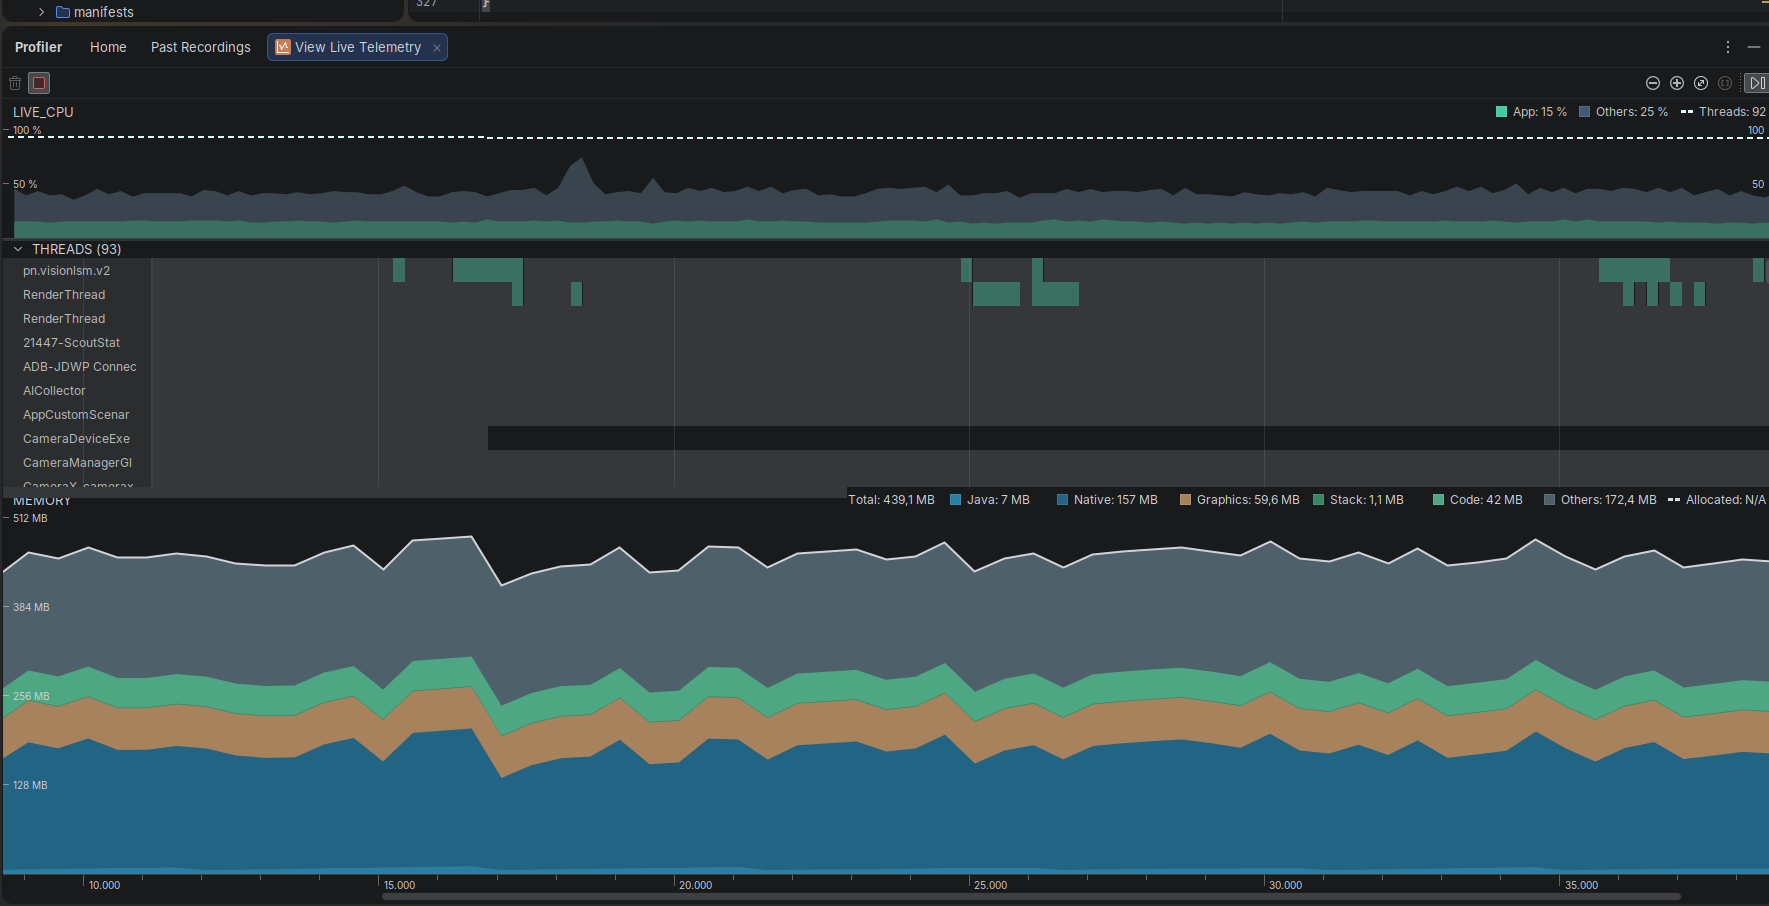
\includegraphics[width=\linewidth]{images/as.png}
		\caption{Monitoreo de CPU, memoria e hilos en inferencia continua utilizando Android Studio Profiler.}
		\label{fig:profiler_android_1}
	\end{figure}
	
	\begin{figure}[H]
		\centering
		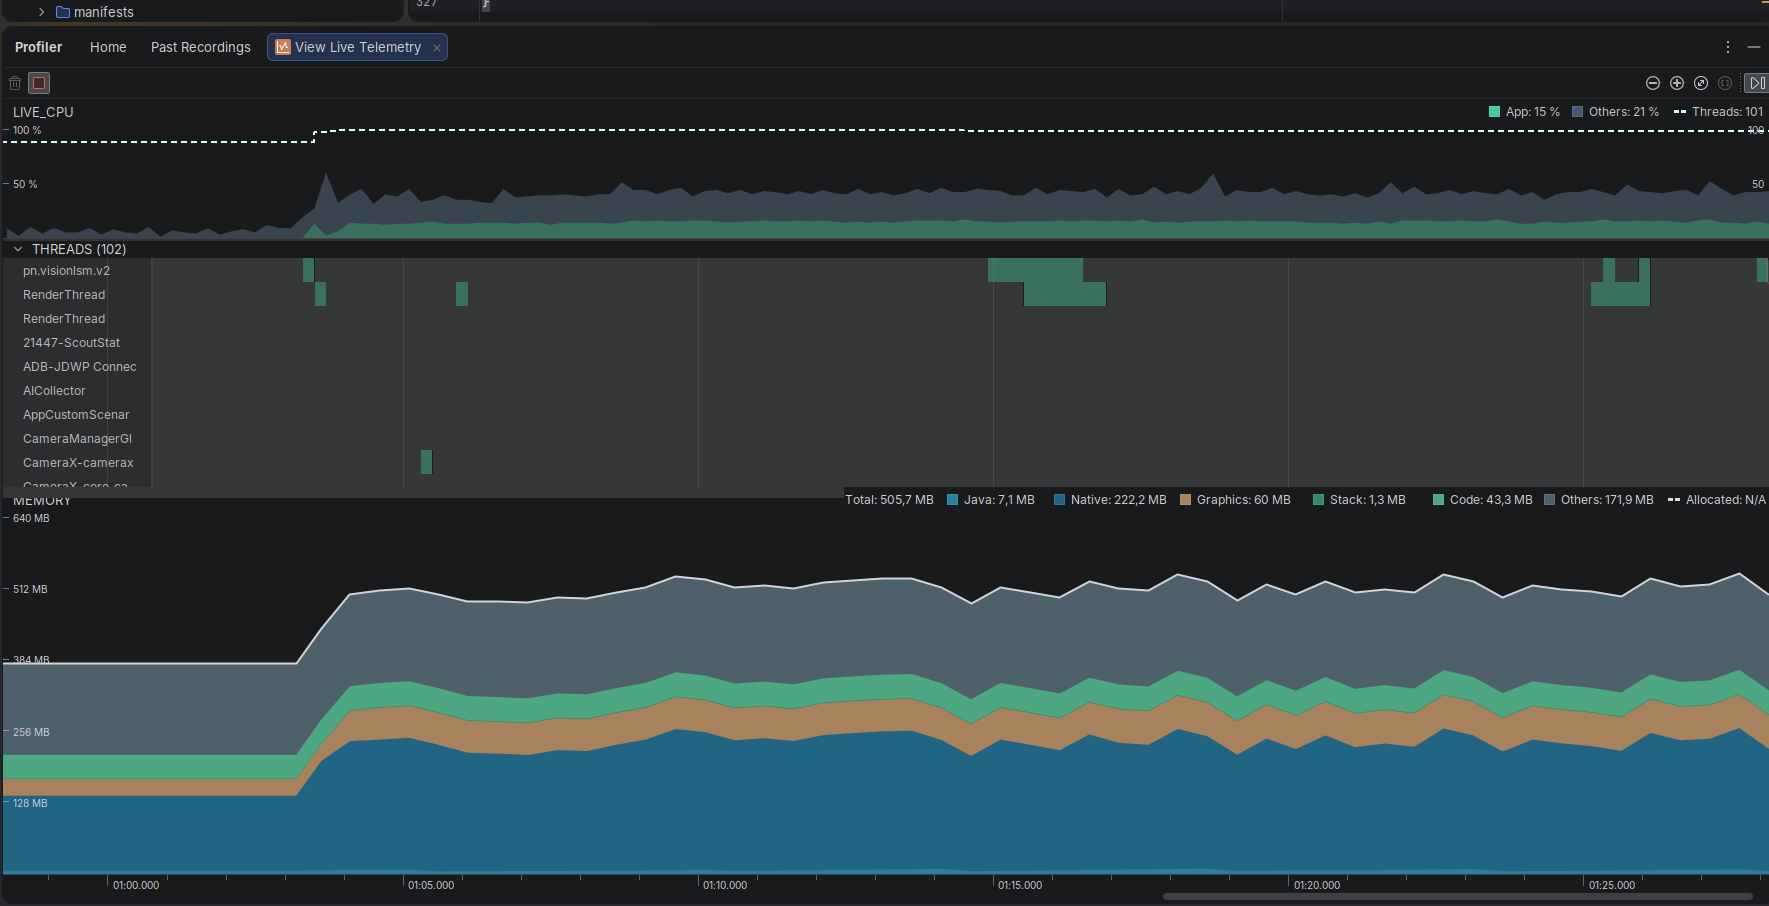
\includegraphics[width=\linewidth]{images/as1.png}
		\caption{Comportamiento estable del consumo de memoria y CPU en ejecución prolongada del prototipo móvil.}
		\label{fig:profiler_android_2}
	\end{figure}
	
	Adicional a las pruebas anteriores se realizó una prueba básica de consumo energético ejecutando la aplicación en aproximadamente 30 minutos de uso continuo. Durante este periodo el dispositivo presentó una disminución cercana al 9\% de batería, incluyendo captura permanente de cámara, procesamiento de landmarks e inferencia local continua.
	
	Aunque estas pruebas no corresponden a un benchmark energético exhaustivo, los resultados obtenidos sugieren que el prototipo mantiene un comportamiento razonable para un sistema de visión por computadora ejecutado completamente de forma local en Android.

	
	
	\subsection{Desarrollo de la interfaz gráfica}
	
	Ademas de los módulos desarrollados y explicados anteriormente, el prototipo necesitaba el desarrollo de una interfaz gráfica que permitiera interactuar con el sistema de reconocimiento de señas. Debido a que la aplicación está orientada a dispositivos móviles, la interfaz debía integrarse directamente con la cámara, mostrar retroalimentación visual y permitir navegación entre los distintos módulos.
	
	El desarrollo de la interfaz se realizó utilizando Jetpack Compose, implementando una estructura basada en pantallas independientes y navegación declarativa. La aplicación incluye vistas para autenticación, pantalla principal, reconocimiento de señas y diccionario visual, además de distintos elementos de retroalimentación visual sobre la cámara.
	
	Dado a que el usuario interactúa simultáneamente con la cámara y el sistema de reconocimiento, se buscó mantener una distribución visual clara, minimizar elementos innecesarios en pantalla y facilitar la interpretación inmediata de los resultados generados por el clasificador.
	
	\subsubsection{Uso de Jetpack Compose}
	
	La interfaz gráfica del prototipo fue desarrollada utilizando Jetpack Compose, el framework moderno de Android para construcción declarativa de interfaces. Esta tecnología permitió diseñar las distintas pantallas de la aplicación mediante componentes reutilizables y estados reactivos, facilitando la integración entre la interfaz visual y el flujo de inferencia del sistema.
	
	A diferencia del enfoque tradicional basado en archivos XML y manipulación manual de vistas, Jetpack Compose utiliza un modelo declarativo donde la interfaz se actualiza automáticamente cuando cambia el estado de la aplicación. Esto ayuda al prototipo desarrollado, debido a que el sistema requiere modificar continuamente elementos visuales mientras la cámara permanece activa y las predicciones cambian constantemente.
	
	La arquitectura general de navegación se implementó mediante \texttt{NavHost} y \texttt{NavController}, centralizando las rutas principales dentro del componente \texttt{AppNavGraph}. Desde este componente se gestionan las distintas pantallas de la aplicación, incluyendo Splash, Login, Home, Cámara y Diccionario.
	
	\begin{lstlisting}[language=Java]
		NavHost(
		navController = navController,
		startDestination = AppDestinations.SPLASH
		)
	\end{lstlisting}
	
	
	Cada pantalla fue implementada como un composable independiente. Por ejemplo, la pantalla principal utiliza el componente \texttt{HomeScreen}, mientras que el módulo de reconocimiento utiliza \texttt{CameraScreen} y el diccionario utiliza \texttt{DictionaryScreen}.
	
	\begin{lstlisting}[language=Java]
		composable(AppDestinations.CAMERA) {
			CameraScreen(navController = navController)
		}
		
		composable(AppDestinations.DICTIONARY) {
			DictionaryScreen(navController = navController)
		}
	\end{lstlisting}
	
	Así se facilita tanto la depuración como el mantenimiento del código. También cada pantalla puede evolucionar de forma relativamente independiente sin modificar el resto de la navegación de la aplicación.
	
	Otra ventaja de Jetpack Compose fue la facilidad para integrar retroalimentación visual dinámica. Debido a que el reconocimiento de señas genera resultados continuamente, era necesario actualizar elementos de interfaz constantemente, como la letra detectada, la confianza de clasificación y los cuadros delimitadores sobre la imagen de cámara. Compose facilita este comportamiento mediante recomposición automática de componentes visuales cuando cambian los estados asociados.
	
	Se utilizo una distribución visual con botones de gran tamaño, paneles claramente diferenciados y colores de alto contraste para mejorar la legibilidad sobre la vista de cámara.
	
	En la pantalla principal se implementó una tarjeta interactiva para iniciar el intérprete de señas y accesos secundarios para herramientas complementarias como el diccionario visual.
	
	\begin{lstlisting}[language=Java]
		Surface(
		modifier = Modifier
		.fillMaxWidth()
		.height(210.dp)
		.clickable {
			navController.navigate(
			AppDestinations.CAMERA
			)
		}
		)
	\end{lstlisting}
	
	Compose también permite construir overlays visuales sobre la cámara utilizando contenedores como \texttt{Box}, facilitando la superposición de información gráfica encima de la vista previa capturada por CameraX para mostrar cuadros delimitadores, estados del sistema y retroalimentación visual sin abandonar la pantalla principal de reconocimiento.
	
	Conforme se realizaron pruebas, fue posible reorganizar componentes, modificar tamaños, adaptar distribuciones verticales y mejorar la compatibilidad con diferentes orientaciones de pantalla sin reestructurar completamente la interfaz.
		
	\subsubsection{Implementación de la pantalla de reconocimiento}
	
	La pantalla de reconocimiento implementada mediante el componente
	\texttt{CameraScreen} representa el núcleo del prototipo,
	ya que en esta vista convergen simultáneamente el sistema de captura
	de imágenes, la detección de landmarks, el procesamiento geométrico
	de la mano y la inferencia del modelo de clasificación.
	
	A diferencia de otras pantallas de la aplicación, esta interfaz mantiene
	un flujo continuo de procesamiento mientras la cámara permanece activa.
	Entonces la pantalla no solamente funciona como una interfaz visual,
	sino también como un componente coordinador entre CameraX, MediaPipe,
	TensorFlow Lite y la lógica interna de captura de señas.
	
	La estructura general de la pantalla se encuentra compuesta por los
	siguientes módulos principales:
	
	\begin{itemize}
		\item Captura de video mediante CameraX.
		\item Vista previa utilizando \texttt{PreviewView}.
		\item Analizador de frames implementado con \texttt{LsmAnalyzer}.
		\item Clasificador TensorFlow Lite mediante \texttt{LsmClassifier}.
		\item Máquina de estados para estabilización de señas.
		\item Elementos visuales superpuestos sobre la cámara.
	\end{itemize}
	
	Primero se verifica que la aplicación cuente con permisos de acceso
	a la cámara. En caso contrario, el sistema solicita dinámicamente dicho
	permiso utilizando \texttt{ActivityResultContracts}.
	
	\begin{lstlisting}[language=Java]
		permissionLauncher.launch(Manifest.permission.CAMERA)
	\end{lstlisting}
	
	Luego se inicializa el componente \texttt{PreviewView},
	encargado de mostrar continuamente la imagen proveniente de la cámara
	frontal del dispositivo.
	
	\begin{lstlisting}[language=Java]
		val previewView = PreviewView(context).apply {
			implementationMode =
			PreviewView.ImplementationMode.COMPATIBLE
			
			scaleType = PreviewView.ScaleType.FILL_CENTER
		}
	\end{lstlisting}
	
	La utilización de \texttt{FILL\_CENTER} permitió mantener la imagen
	ocupando completamente la pantalla, aunque esto también introdujo
	problemas relacionados con el escalado y la relación de aspecto,
	los cuales posteriormente requirieron funciones adicionales de
	mapeo geométrico para posicionar correctamente las cajas delimitadoras.
	
	El sistema de inferencia es inicializado mediante el componente
	\texttt{LsmClassifier}, encargado de cargar el modelo TensorFlow Lite
	y las etiquetas correspondientes al alfabeto reconocido.
	
	\begin{lstlisting}[language=Java]
		val classifier = LsmClassifier(
		context = context,
		modelAssetPath = "models/model_lsm_v3.tflite",
		labelsAssetPath = "models/labels.txt"
		)
	\end{lstlisting}
	
	De manera paralela se implementó una máquina de estados denominada
	\texttt{SignCaptureStateMachine}, cuya función consiste en estabilizar
	las predicciones generadas por el modelo.
	
	\begin{lstlisting}[language=Java]
		val stateMachine = SignCaptureStateMachine(
		minConfidence = 0.55f,
		stableTimeMs = 200L,
		flashDurationMs = 150L
		)
	\end{lstlisting}
	
	Esta lógica evita confirmar letras inestables producidas por falsos
	positivos momentáneos, exigiendo que la predicción permanezca estable
	en un intervalo mínimo antes de incorporarse al texto final.
	
	La captura y procesamiento de imágenes se realiza utilizando CameraX
	mediante dos componentes principales: \texttt{Preview} e
	\texttt{ImageAnalysis}.
	
	\begin{lstlisting}[language=Java]
		val preview = Preview.Builder()
		.setTargetAspectRatio(
		AspectRatio.RATIO_16_9
		)
		.build()
	\end{lstlisting}
	
	Mientras \texttt{Preview} se encarga de mostrar la imagen en pantalla,
	el componente \texttt{ImageAnalysis} permite procesar cada frame
	capturado por la cámara.
	
	\begin{lstlisting}[language=Java]
		val imageAnalysis = ImageAnalysis.Builder()
		.setTargetResolution(Size(1280, 720))
		.setBackpressureStrategy(
		ImageAnalysis.STRATEGY_KEEP_ONLY_LATEST
		)
		.build()
	\end{lstlisting}
	
	La estrategia \texttt{KEEP\_ONLY\_LATEST} fue importante para evitar
	acumulación de frames pendientes en la inferencia. En lugar de
	procesar todos los frames capturados, el sistema descarta automáticamente
	los frames atrasados y conserva únicamente el más reciente, reduciendo
	latencia y manteniendo estabilidad en la ejecución continua.
	
	El procesamiento de cada frame es delegado al componente
	\texttt{LsmAnalyzer}, encargado de transformar las imágenes capturadas
	en landmarks compatibles con el modelo de clasificación.
	
	\begin{lstlisting}[language=Java]
		it.setAnalyzer(cameraExecutor, analyzer)
	\end{lstlisting}
	
	Dentro del analizador, cada frame recibido es convertido inicialmente
	desde \texttt{ImageProxy} hacia un objeto \texttt{Bitmap}. Posteriormente
	se aplican transformaciones geométricas para corregir la orientación
	reportada por Android y el efecto espejo generado por la cámara frontal.
	
	\begin{lstlisting}[language=Java]
		matrix.postRotate(
		imageInfo.rotationDegrees.toFloat()
		)
		
		matrix.postScale(-1f, 1f)
	\end{lstlisting}
	
	Estas correcciones fueron necesarias debido a que pequeñas variaciones
	de orientación podían modificar significativamente la distribución espacial
	de los landmarks detectados por MediaPipe, afectando directamente el
	comportamiento del modelo.
	
	Despues de corregir la imagen, ésta es enviada al detector de MediaPipe
	Hands mediante el método \texttt{detectForVideo()}, permitiendo obtener
	los 21 landmarks correspondientes a la mano detectada.
	
	Posteriormente se construye el vector de características compuesto por
	42 valores numéricos correspondientes a las coordenadas \texttt{x} y
	\texttt{y} de cada landmark.
	
	La normalización implementada utiliza el ancho y alto de la mano para
	normalizar independientemente cada eje, reduciendo la dependencia
	respecto a escala, posición y distancia de la mano dentro del encuadre.
	
	\[
	x_i' =
	\frac{x_i - \min(x)}{w}
	\]
	
	\[
	y_i' =
	\frac{y_i - \min(y)}{h}
	\]
	
	El resultado generado por el clasificador es  enviado hacia
	la interfaz gráfica, actualizando dinámicamente la letra detectada,
	el porcentaje de confianza, el progreso de estabilización y las cajas
	delimitadoras mostradas sobre la vista previa.
	
	Para mejorar la experiencia visual se incorporaron animaciones mediante
	\texttt{animateFloatAsState()}, permitiendo suavizar el movimiento de
	las cajas delimitadoras y las barras de progreso mostradas en la
	captura de señas.
	La pantalla incorpora distintos modos de distribución
	adaptativa dependiendo de la orientación y tamaño del dispositivo,
	incluyendo configuraciones específicas para orientación vertical,
	horizontal y tabletas.
	
	Por ultimo se implementó una capa de depuración visual denominada
	\texttt{DEBUG MODE}, utilizada en las pruebas experimentales para
	mostrar tiempos de inferencia, confianza de clasificación y etiquetas
	detectadas de forma continua.

	
	\subsection{Implementación de la máquina de estados}
	
	Uno de los retos mas complicados consistió en mantener estabilidad en el reconocimiento continuo de señas. Debido a que la aplicación realiza clasificación de señas de manera constante sobre los frames capturados por la cámara, las predicciones pueden variar ligeramente entre cuadros consecutivos como consecuencia de pequeños movimientos de la mano, variaciones geométricas, fluctuaciones en los landmarks o cambios momentáneos en la confianza del modelo.
	
	Si cada predicción obtenida fuese aceptada inmediatamente, el sistema produciría múltiples capturas incorrectas, repeticiones accidentales de letras y escritura inestable dentro de la interfaz. Para mitigar estos problemas se implementó una máquina de estados encargada de controlar el flujo completo de reconocimiento, validación temporal, confirmación y liberación de señas.
	
	La lógica fue desarrollada mediante la clase \texttt{SignCaptureStateMachine}, la cual administra los distintos estados internos del proceso de captura y mantiene sincronizada la interacción entre el reconocimiento, la interfaz gráfica y la construcción dinámica del texto generado por el usuario.
	
	El sistema implementa cuatro estados principales:
	
	\begin{itemize}
		\item \textbf{IDLE}: estado de espera donde el sistema permanece hasta detectar una seña válida.
		
		\item \textbf{DETECTING}: estado temporal donde la aplicación verifica que la seña permanezca estable en un intervalo mínimo de tiempo.
		
		\item \textbf{CONFIRMED\_FLASH}: estado utilizado para mostrar visualmente que la seña fue capturada correctamente.
		
		\item \textbf{WAITING\_RELEASE}: estado que evita múltiples capturas consecutivas de la misma seña mientras la mano continúa visible frente a la cámara.
	\end{itemize}
	
	La transición entre estados permite controlar el reconocimiento continuo de forma más estable y reducir considerablemente falsos positivos, repeticiones accidentales y fluctuaciones momentáneas en las predicciones generadas por el modelo.
	
	La máquina de estados administra distintos elementos de retroalimentación visual dentro de la interfaz, incluyendo mensajes dinámicos, barras de progreso, confirmaciones visuales y la construcción progresiva del texto reconocido.
	
	La Figura~\ref{fig:diagrama_maquina_estados} muestra el flujo general implementado para el proceso de captura y validación temporal de señas dentro del prototipo móvil.
	
	\begin{figure}[H]
		\centering
		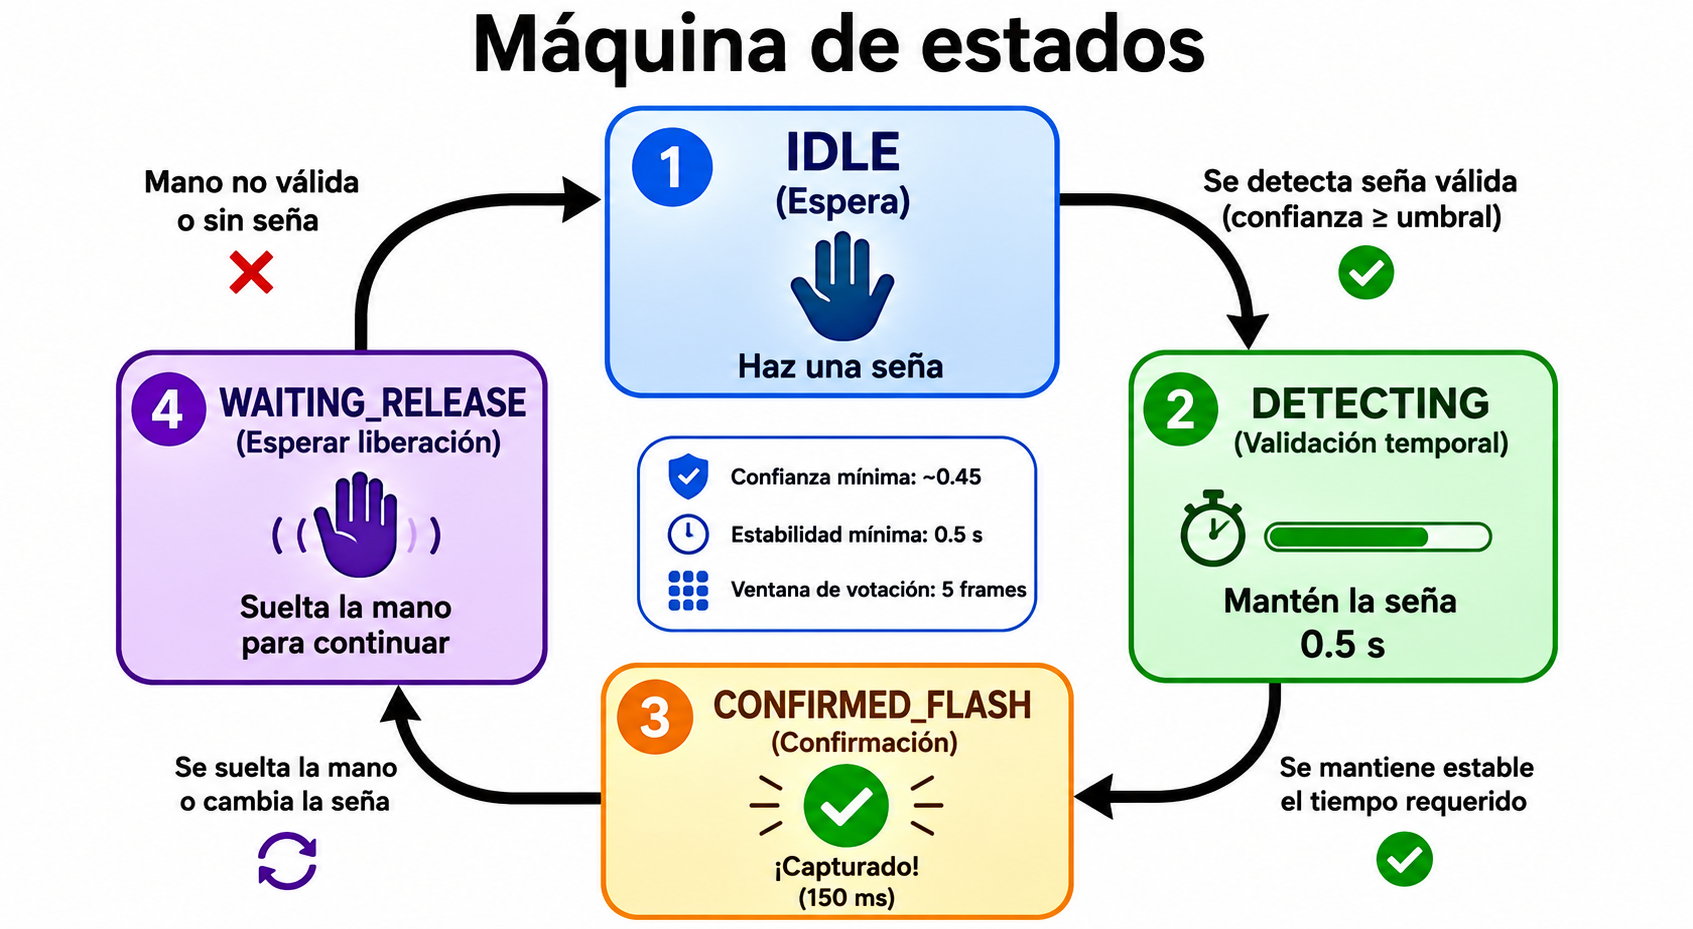
\includegraphics[width=0.95\linewidth]{images/FSM.png}
		\caption{Máquina de estados implementada para el control del reconocimiento continuo y la captura de señas dentro de la aplicación móvil.}
		\label{fig:diagrama_maquina_estados}
	\end{figure}
	
	\subsubsection{Validación temporal y estabilidad del reconocimiento}
	
	Dado que el prototipo realiza clasificaciones m continua sobre los frames capturados por la cámara, las predicciones generadas por el modelo pueden presentar pequeñas fluctuaciones temporales entre cuadros consecutivos. Estas variaciones pueden producirse como consecuencia de movimientos naturales de la mano, cambios mínimos en la geometría detectada por MediaPipe Hands o variaciones momentáneas en la confianza de clasificación.
	
	Si cada predicción fuese aceptada inmediatamente, el sistema produciría múltiples capturas incorrectas, escritura inestable y falsas detecciones en el reconocimiento continuo. Para reducir este problema se implementó un mecanismo de validación temporal basado en persistencia de la seña y votación por mayoría dentro de una ventana deslizante de predicciones.
	
	Cada predicción generada por el modelo es validada mediante un umbral mínimo de confianza definido dentro de la máquina de estados:
	
	\begin{lstlisting}[language=java]
		private val minConfidence: Float = 0.45f
	\end{lstlisting}
	
	Únicamente las predicciones cuya confianza supera dicho umbral son consideradas válidas para el proceso de reconocimiento. Posteriormente, las etiquetas válidas son almacenadas temporalmente dentro de una ventana de predicciones recientes:
	
	\begin{lstlisting}[language=java]
		private val windowSize: Int = 5
	\end{lstlisting}
	
	La ventana deslizante permite mantener un historial corto de predicciones consecutivas y aplicar un proceso de votación por mayoría. Así es como el sistema selecciona únicamente la etiqueta dominante dentro de los últimos frames analizados, reduciendo fluctuaciones instantáneas y aumentando la estabilidad temporal del reconocimiento.
	
	La seña detectada debe mantenerse estable en un intervalo mínimo antes de ser aceptada por el sistema:
	
	\begin{lstlisting}[language=java]
		private val stableTimeMs: Long = 200L
	\end{lstlisting}
	
	Mientras la seña permanece estable, la interfaz gráfica muestra una barra de progreso que indica visualmente el avance del proceso de validación temporal. Una vez transcurrido el tiempo requerido y manteniéndose la misma seña dominante dentro de la ventana de votación, la máquina de estados considera que la predicción es suficientemente estable para ser confirmada.
	
	De esta forma se redujo considerablemente falsos positivos, variaciones abruptas entre frames y capturas accidentales en el reconocimiento continuo de señas en el dispositivo móvil.
	
	\subsubsection{Confirmación de señas y construcción de texto}
	
	Cuando la máquina de estados determina que una seña permanece estable en el intervalo de validación temporal, el sistema procede a confirmar oficialmente la predicción y agregarla al texto construido dentro de la interfaz.
	
	La confirmación ocurre cuando la misma etiqueta dominante se mantiene estable en el tiempo mínimo definido por la variable \texttt{stableTimeMs}. En ese momento, la letra reconocida es concatenada automáticamente al texto acumulado por el usuario:
	
	\begin{lstlisting}[language=java]
		confirmedText += winningLabel
	\end{lstlisting}
	
	Luego el sistema almacena temporalmente la última seña confirmada con la finalidad de evitar duplicados accidentales durante el reconocimiento continuo:
	
	\begin{lstlisting}[language=java]
		lastConfirmedLabel = winningLabel
	\end{lstlisting}
	
	Después de capturar una letra, la máquina de estados entra en el estado \texttt{WAITING\_RELEASE}, donde el sistema espera a que la mano desaparezca parcialmente del área de captura o a que el usuario cambie de configuración manual antes de permitir una nueva detección. Esta lógica evita que una misma seña sea escrita repetidamente mientras el usuario mantiene la mano frente a la cámara.
	
	La transición de liberación se realiza mediante la siguiente validación:
	
	\begin{lstlisting}[language=java]
		if (winningLabel == null ||
		winningLabel == "?" ||
		winningLabel != lastConfirmedLabel)
	\end{lstlisting}
	
	El sistema únicamente regresa al estado de detección cuando la seña cambia o desaparece, permitiendo una escritura mucho más controlada y estable en el reconocimiento continuo.
	
	La aplicación incorpora funciones complementarias para la construcción dinámica de texto, incluyendo inserción manual de espacios y eliminación de caracteres previamente capturados:
	
	\begin{lstlisting}[language=java]
		fun addSpace()
		
		fun deleteLast()
	\end{lstlisting}
	
	Estas funciones permiten que el usuario pueda construir palabras y frases progresivamente mediante secuencias consecutivas de señas reconocidas por el sistema.
	
	Esta lógica permitió transformar el reconocimiento individual de letras en un flujo continuo de escritura , manteniendo estabilidad temporal y reduciendo considerablemente repeticiones accidentales durante la interacción con la aplicación móvil.
	
	\subsubsection{Retroalimentación visual y experiencia de interacción}
	
	Otro de los aspectos considerados en el desarrollo del prototipo fue la interacción visual entre el sistema y el usuario. Debido a que la aplicación realiza reconocimiento continuo, era necesario proporcionar indicadores visuales claros que permitieran comprender el estado actual del proceso de captura y validación de señas.
	
	La interfaz incorpora distintos mecanismos de retroalimentación visual controlados directamente por la máquina de estados. Cada estado interno modifica dinámicamente mensajes, colores, efectos visuales y barras de progreso para comunicar al usuario el estado actual del reconocimiento.
	
	Los mensajes principales utilizados en la interacción son:
	
	\begin{itemize}
		\item \textbf{Haz una seña}: indica que el sistema se encuentra esperando una detección válida.
		
		\item \textbf{Mantén la seña}: aparece mientras la aplicación realiza la validación temporal de estabilidad.
		
		\item \textbf{¡Capturado!}: confirma visualmente que la seña fue reconocida correctamente.
		
		\item \textbf{Suelta para continuar}: evita capturas repetidas mientras la misma seña permanece frente a la cámara.
	\end{itemize}
	

	
	En el estado de detección se muestra una barra de progreso dinámica que representa visualmente el tiempo restante necesario para validar la estabilidad de la seña. Este mecanismo permite que el usuario comprenda cuándo una predicción está siendo procesada y reduce la sensación de incertidumbre en la interacción.
	
	La interfaz también incorpora efectos visuales de confirmación mediante iluminación temporal (\textit{glow}) y cambios de estado visuales una vez que una letra es capturada exitosamente. Estos elementos ayudan a mejorar la claridad del flujo de interacción y proporcionan confirmaciones inmediatas sin necesidad de interrumpir el reconocimiento continuo.
	
	Estos mecanismos permitieron construir una experiencia de interacción más estable, intuitiva y comprensible para el usuario, reduciendo errores de captura y facilitando el uso continuo del sistema dentro del dispositivo móvil.
	
	La Figura~\ref{fig:fsm_feedback} muestra algunos ejemplos del funcionamiento visual implementado en el proceso de reconocimiento continuo dentro de la aplicación móvil.
	
	\begin{figure}[H]
		\centering
		
		\begin{subfigure}[b]{0.32\linewidth}
			\centering
			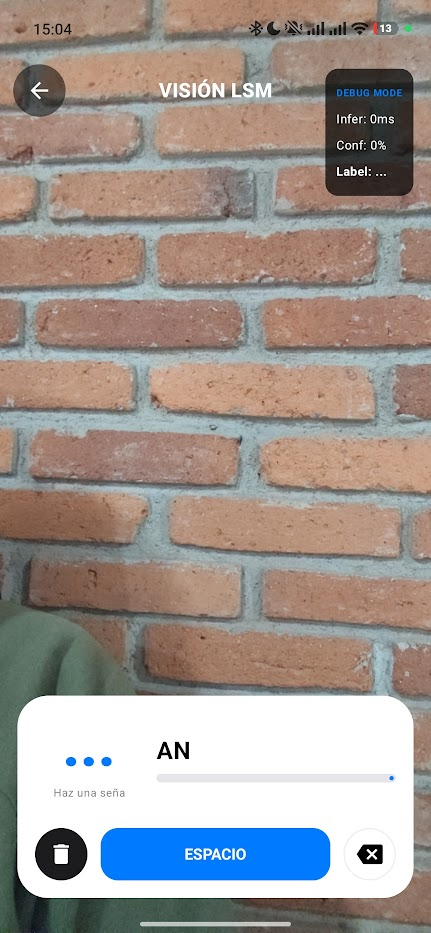
\includegraphics[width=\linewidth]{images/idle.png}
			\caption{Estado de espera}
		\end{subfigure}
		\hfill
		\begin{subfigure}[b]{0.32\linewidth}
			\centering
			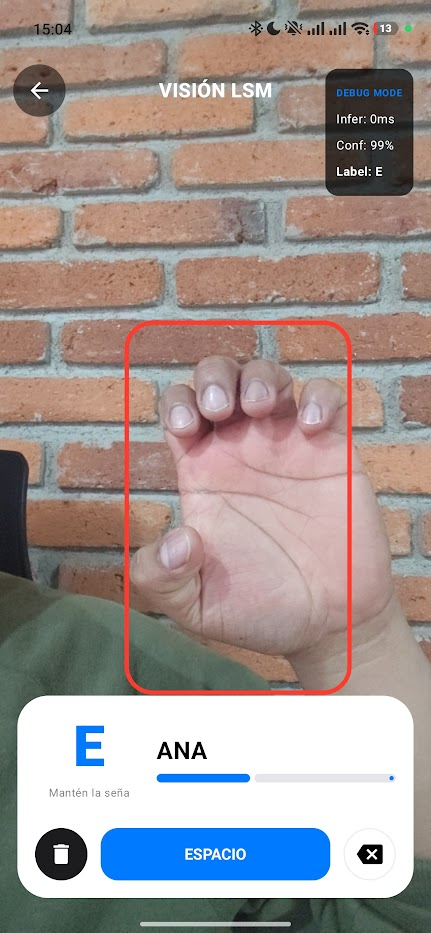
\includegraphics[width=\linewidth]{images/confirmando.png}
			\caption{Validación temporal}
		\end{subfigure}
		\hfill
		\begin{subfigure}[b]{0.32\linewidth}
			\centering
			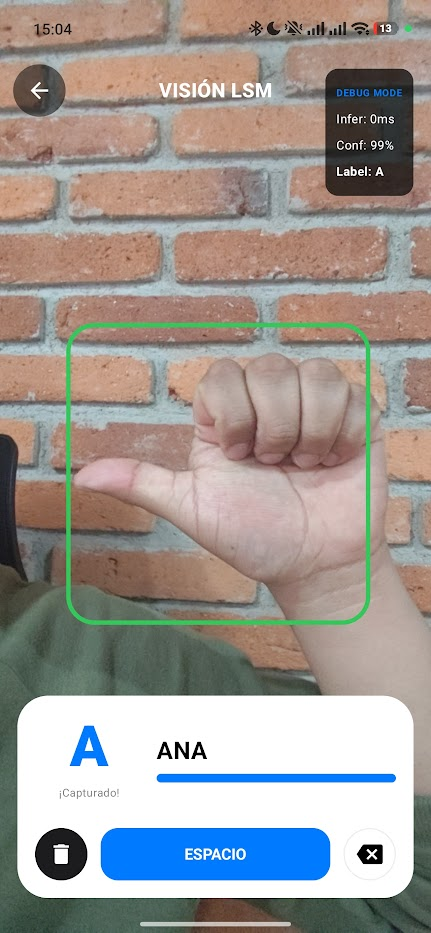
\includegraphics[width=\linewidth]{images/confirmado.png}
			\caption{Captura confirmada}
		\end{subfigure}
		
		\caption{Retroalimentación visual implementada en las distintas etapas del reconocimiento continuo de señas.}
		\label{fig:fsm_feedback}
	\end{figure}
	
	En la Figura~\ref{fig:fsm_feedback}(a) el sistema se encuentra en estado de espera (\texttt{IDLE}), por lo que no existe una seña válida detectada dentro del área de captura. En esta etapa la interfaz muestra el mensaje ``Haz una seña'', indicando que el sistema permanece listo para iniciar un nuevo proceso de reconocimiento.
	
	Luego la Figura~\ref{fig:fsm_feedback}(b) muestra el estado de validación temporal (\texttt{DETECTING}). En este caso el sistema ya detectó una posible seña y comienza el proceso de estabilización temporal antes de aceptarla definitivamente. En esta etapa se activa la barra de progreso y el mensaje ``Mantén la seña'', indicando al usuario que debe conservar la configuración de la mano en un breve intervalo para confirmar la predicción.
	
	Y por último la Figura~\ref{fig:fsm_feedback}(c) corresponde al estado de confirmación (\texttt{CONFIRMED\_FLASH}), donde la seña ya fue aceptada por la máquina de estados y agregada dinámicamente al texto construido por el usuario. En esta etapa el cuadro de captura cambia visualmente a color verde y aparece el mensaje ``¡Capturado!'', proporcionando retroalimentación inmediata sobre el reconocimiento exitoso de la letra detectada.
	

	\newpage
